\pagestyle{empty}
\cleardoublepage
\pagestyle{fancy}

\selectlanguage{english}


\chapter{Genetic Architecture and the Evolution of Variational Modularity}

Diogo Melo, Eleanor O'Brien, John Hunt, Jason Wolf, Gabriel Marroig

\newpage

\vspace*{10pt}
% Abstract
\begin{center}
  \emph{\begin{large}Abstract\end{large}}
\vspace{2pt}
\end{center}

\noindent
Genetic architecture interacts with the evolutionary processes and is a key
factor in determining short and long-term evolution. For a set of traits, the
evolutionary response to selection and expected outcome of multivariate drift
depend on the pattern of genetic covariation. Ultimately, genetic covariation
is determined by genetic architecture and allelic variation, and we hope to
understand how genetic architecture can influence evolution by studying
covariation.  However, it is not clear how closely additive genetic
covariation reflects the underlying genotype-phenotype map, as several GP-maps
can lead to the same pattern of covariation. We use an explicit individual-
based simulation approach to investigate how genetic effects evolve under
different selection regimes, and how these evolving genetic effects are
reflected in the pattern of covariation. We confront these computational
results with multivariate mapping of genetic effects in an experimental
population of mice composed from lineages derived by artificial selection. We
estimate the multivariate effect of loci on growth and use these effect
‘vectors’ to examine how pleiotropy in the genotype-phenotype map determines
genetic covariance structure. We show that under simulations and in real
populations the covariance pattern is determined by a complex combination of
different types of genetic effects that interact to determine the pattern of
covariation.
\par
\vspace{1em}
\noindent\textbf{Keywords:} G-matrix; QTL mapping; genome prediction; genetic architecture
\newpage

\begin{refsection}


\section{Introduction}

Heritable genetic variation determines a trait's evolvability, defined as the
ability to respond to selection. In order to efficiently respond to selection,
traits must have enough genetic variation to change under selection, and this
variation must be somewhat independent from the rest of the
organism~\parencite{Lewontin1979-iw}. Genetic correlations captures the
pattern of genetic dependency between traits~\parencite{Lande1979-by,
Lande1983-ez} and a modular variational pattern, in which functionally related
traits are more correlated while being less correlated with other traits,
provides an organization that permits groups of traits to evolve in a
coordinated fashion while not disturbing other traits~\parencite{Olson1958-qk,
Cheverud1996-jw, Wagner2007-cx, Melo2016-yw}.

The genetic association between traits is largely determined by the
pleiotropic relations between alleles and phenotypes, and shared development,
both of which are summarized in the genotype-phenotype map. If pleiotropic
effects are mostly synergistic with respect to phenotypes, affecting trait
means in the same direction, traits that share more pleiotropic effects will
be more correlated, while traits that share few effects will be less
correlated. This leads to the hypothesis that the variational modularity we
observe in the population is generated by a particular type of GP map, in
which the genetic effects themselves are modular and restricted to a limiter
number of related traits~\parencite{Wagner1996-ui}. Indeed, some degree of
modularity in the organization of genetic effects has often been shown to
underlie modular variation~\parencite{Cheverud1997-rw, Mezey2000-rs, Kenney-
Hunt2008-bd, Porto2016-qc, Leamy1999-dm}. However, the relation between
pleiotropy and covariation is complicated by a many-to-one mapping between
pleiotropy and variational modularity~\parencite{Mitteroecker2009-jb}. A
modular GP map is not a prerequisite for variational modularity, as pleiotropic
effects can also affect two traits or modules in opposite directions, creating
antagonistic pleiotropy. Antagonistic pleiotropy can generate variational
modularity by canceling out synergistic pleiotropic effects, and in doing so
reduce genetic correlations, a process known as hidden
pleiotropy~\parencite{Turelli1985-ne, Pavlicev2011-xm}. While hidden
pleiotropy can allow traits to be uncorrelated while sharing allelic effects,
it can still constrain the evolution of uncorrelated
traits~\parencite{Baatz1997-hh}. If we consider non-linear GP maps, the
situation is even more complex, as the mean pleiotropic effect also has the
potential do change the covariance pattern~\parencite{Mitteroecker2009-jb}.

When considering the effects of the GP map on
evolvability,~\textcite{Hansen2003-fh} points out that evolvability can be
attained from genetic architectures other than a modular one, and that
independence between traits must be balanced with the allelic effects needed
to provide variation. That is, less shared allelic effects between
traits leads to the modular variation that allows the traits to evolve
independently, but more shared allelic effects increases the amount of
available variation for selection. A GP map that maximizes
evolvability must be somewhere in between, providing both independence between
traits and variability for each trait. If we allow antagonistic pleiotropy,
then a GP map with all genes affecting all traits can be modular and maximally
evolvable. Antagonistic pleiotropy allows generalized pleiotropic effect to
produce modular variation while still contributing to trait
variance.~\textcite{Hansen2003-fh} and~\textcite{Pavlicev2011-xm} explore the
conditions under which highly modular or highly pleiotropic GP maps provide
higher conditional evolvability, defined as the variation available to respond
to directional selection in one trait when the other traits are under
stabilizing selection. In a two trait system, the two extreme architectures
can both evolve when we consider directional selection on one trait and
stabilizing selection on the other. If stabilizing selection is stronger, the
modular architecture is favored since the penalty for correlated response is
higher and the modular system provides a smaller unit of selection. If
directional selection is stronger than stabilizing selection, the added per
trait genetic variance from additional pleiotropic effects can compensate the
maladaptive correlated response in the trait under stabilizing selection.
Under stabilizing selection on both traits, details of the distribution of
allelic effects and the strength of stabilizing selection on each trait can
determine which genetic architecture provides higher
evolvability~\parencite{Pavlicev2011-xm}. Under high mutation rates and small
mutational effects, the hidden pleiotropy GP map provides higher evolvability,
while under small mutation rates and large mutational effects, the modular GP
map provides higher evolvability.

Conditional evolvability measured on standing genetic variation adequately
describes the short term ability of complex phenotypes to respond to
selection, but longer time scales require us to also consider the influx of
mutational variation, and genetic architecture also affects the long term
effect of mutations. For example, a modular genetic architecture allows
mutational effects to be restricted to functional groups of traits and reduces
the cost of deleterious pleiotropic mutations. In regards to the long term
influence of genetic architecture on the response to selection, we only expect
genetic architecture to constrain long term evolution if it causes mutational
correlation~\parencite{Chebib2017-sv}. Long term evolution also requires us to
understand how genetic architecture evolves. Variation on genetic architecture
has been widely established in recent years, with several works showing the
role epistasis has in providing variation in pleiotropic and variational
patterns~\parencite{Pavlicev2015-up, Cheverud1996-fm, Cheverud2004-qr,
WolF$_{\text{2}}$006-xt, Pavlicev2008-jy}, variation that can then be selected on.
Selection on covariation patterns can be direct, caused by correlated
stabilizing selection~\parencite{Burger1994-nv} which causes the genetic and
mutational variation to align with pattern of
selection~\parencite{Cheverud1984-mi}. Epistatic interactions between additive
loci provide the necessary variation in the pattern of mutational correlations
to allow this alignment to evolve in response to correlated stabilizing
selection~\parencite{Jones2014-wj}. Directional selection can also contribute
to the evolution of covariation, and there is evidence that traits that are
selected together tend to become more correlated, both in
simulations~\parencite{Pavlicev2011-wz, Melo2015-bk, Jones2004-be,
Watson2014-pi} and in natural populations~\parencite{Penna2017-if,
Assis2016-vz, RofF$_{\text{2}}$012-fe}. The effect of directional selection on the
covariance structure can be summarized in the words of Brazilian writer Pedro
Nava: "Experience is a headlight that shines backwards", that is, directional
selection can bias genetic correlation such that there is an increase in the
(relative) evolvability in the directions of past selection. In this sense, we
might think of current pattern of constraints as being adaptations to the
evolutionary history of the population~\parencite{Draghi2008-cv}, although
this hypothesis is controversial~\parencite{Lynch2007-kz, Lynch2007-ch}. There
has also been some effort into directly selecting for changes in the
covariation structure, and response to direct selection in covariation can be
quite dramatic~\parencite{Delph2011-bc}, but we lack a comprehensive picture
for this type of experiment, and we do not know if this type of selective
pressure is common in nature.

The evolution of pleiotropic effects also includes second order constraints on
the variation in pleiotropy. Development imposes internal selection on the
phenotype, in the sense that there is a certain minimum requirement of
producing traits that are compatible with each other. This basic evo-devo
restriction determines which variants are compatible with forming a complete
functioning individual, and can be stable over macro-evolutionary
timescales.~\textcite{Mitteroecker2009-jb} argues that variational modularity
over longer timescales can only be obtained through localized developmental
factors, because over these time-scales the non-linear aspects of development
preclude compensatory pleiotropy from being stable. There is very little
empirical evidence on constraints in the structure of pleiotropic effects, but
see the last chapter and~\textcite{Pavlicev2016-jh} for an example of
development shaping genetic effects.

In this article (chapter?) we use a combination of individual based
simulations and an advanced intercross between inbreed mice to explore the
pleiotropic base of a change in covariation structure. To create the
intercross, we use several inbreed mice lines that were derived from the
directional selection experiment by~\textcite{Atchley1997-vn}. In this
experiment, an initial positive correlation between growth traits within the
initial population was eroded by divergent selection between selected strains.
These selected strains were then inbreed, and using these inbreed lines, we
created an advanced intercross line to investigate the genetic basis of the new
covariance pattern across lines. We confront the results from this
experimental cross with results from simulations. Using an individual based
simulation, we explore how pleiotropic patterns evolve under different
selection regimes. We relate the genetic effects to the observed covariation
in the simulated populations. We expect the pattern of divergent directional
selection to influence the pleiotropic basis of the covariation pattern in
both simulated and experimental populations.


\section{Methods}

\subsection{Simulation model}

We use an individual-based model with a large number (m = 200) of pleiotropic
diploid additive loci controlling four quantitative traits in 5000
hermaphroditic individuals. All loci can potentially affect all traits, and so
the effects of each locus can be represented by a 4-dimensional vector in
trait space (Fig.~\ref{effectvectors}). Individual phenotypes are determined
by adding all allelic effects vectors for each individual, resulting in a
population of 4 dimensional phenotypes. Phenotypes are then used to attribute
a fitness to each individual according to a Gaussian selection surface defined
by a multivariate optimum and a selective covariance matrix. Mating pairs are
sampled with probability proportional to their fitness and gametes formed by
sampling one allele for each locus. Mutation occurs before gamete sampling and
is represented by a small random change in the direction and magnitude of the
allelic effect vector. These two types of changes, in direction and magnitude
of the pleiotropic vector, can occur at different rates~\parencite[for a
discussion on both types of mutations see][]{Draghi2010-ye}. Both mutation
types occur with a fixed per-generation per-loci mutation probability. We use
a mutation probability for the magnitude of the effects of $10^{-4}$ and a
mutation probability in the direction of the effects (the pleiotropy) of
$10^{-5}$, so the pleiotropic pattern changes more slowly than the magnitude
of the effects. Mutations in magnitude are drawn from a normal distribution
with mean zero and variance 0.1 and added to the original vector. Mutations in
direction are drawn from a multivariate normal distribution with zero mean and
a diagonal covariance matrix with variances set to 0.1. In the case of a
mutation in direction, after adding the mutation to the original effect
vector, the resulting vector is scaled to keep the original magnitude. If the
variance of the added vector is small, this produces a small change in the
pattern of pleiotropy. All loci are unlinked and inherited independently.
Correlated stabilizing selection is applied using a selection covariance
matrix with non-zero off-diagonal elements. Directional selection is applied
by using a moving optimum. These selective regimes were chosen because all of
them have been previously implicated in the evolution of variational
modularity in different simulation models~\parencite{Jones2014-wj,
Melo2015-bk}. Both directional selection regimes require some independence
between traits in the two modules, as they must change independently in order
to respond to the applied selective pressure.

We use three selection regimes to investigate the effects of evolutionary
history on the genetic architecture of variational modularity. Populations are
first subjected to several generations of drift, then correlated stabilizing
selection with two modules. Module M1 composed of traits 1 and 2 and Module M2
of traits 3 and 4. Within module correlation in the selective covariance matrix
is set at 0.8, between module is set at zero. After stabilizing selection, in
two of the simulated scenarios, we apply directional selection. We use two
directional selection modes (1) under divergent directional selection the two
modules are selected in opposite directions; (2) under corridor selection, one of
the modules is under directional selection while the other is under stabilizing
selection (Fig.~\ref{selectionregimes}).

\begin{figure}
    \centering
    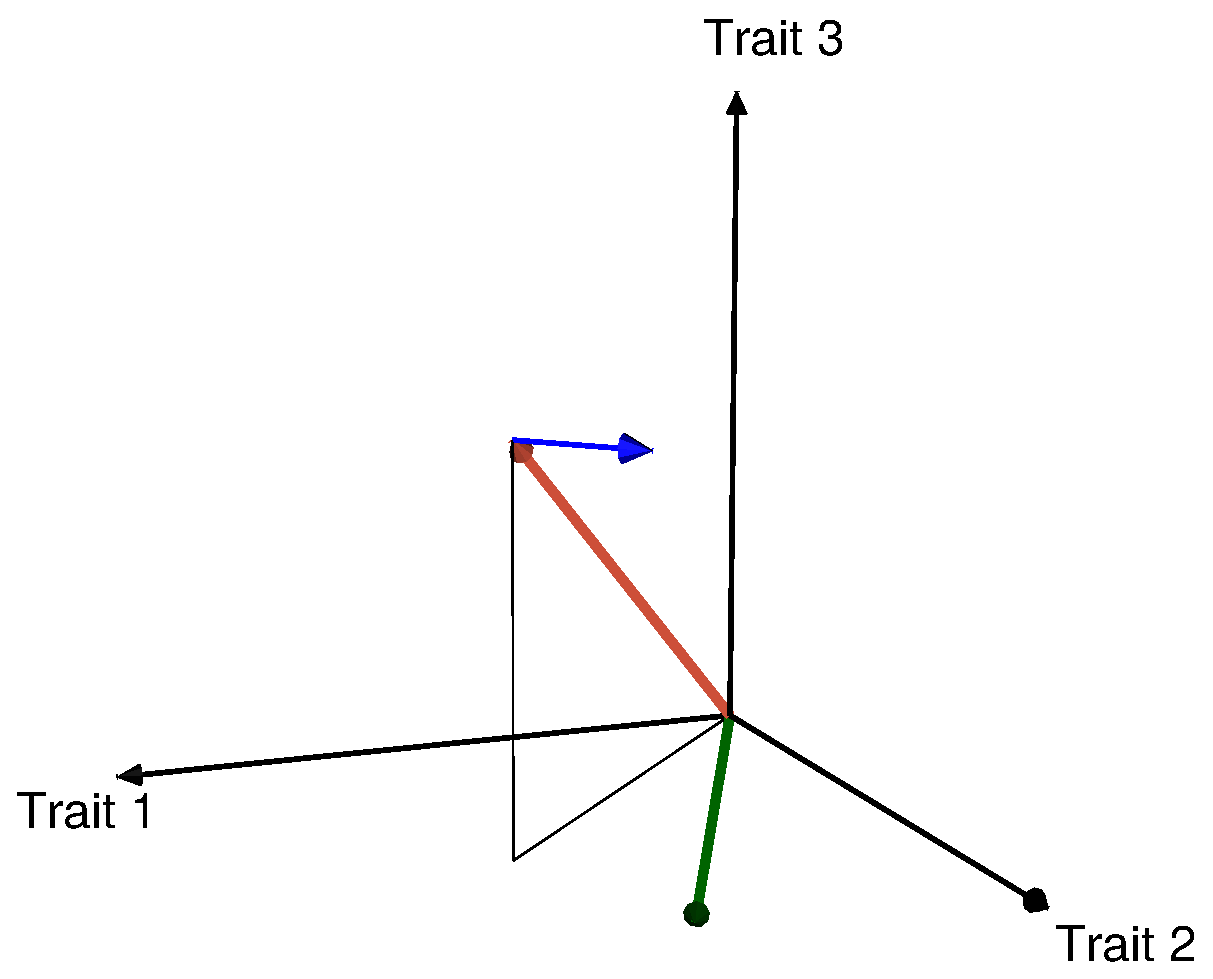
\includegraphics[width=\linewidth]{chapter_atchley/media/plot.eps}
    \caption[Pleiotropic effect in trait space]{Representation of vectors of genetic effects in trait space. Red vector is an integrative vector, while the green vector is modular with respect to traits 1 and 2. Blue vector represents a possible mutation that alters the direction of the red effect.}
    \label{effectvectors}
\end{figure}

\begin{figure}
    \centering
    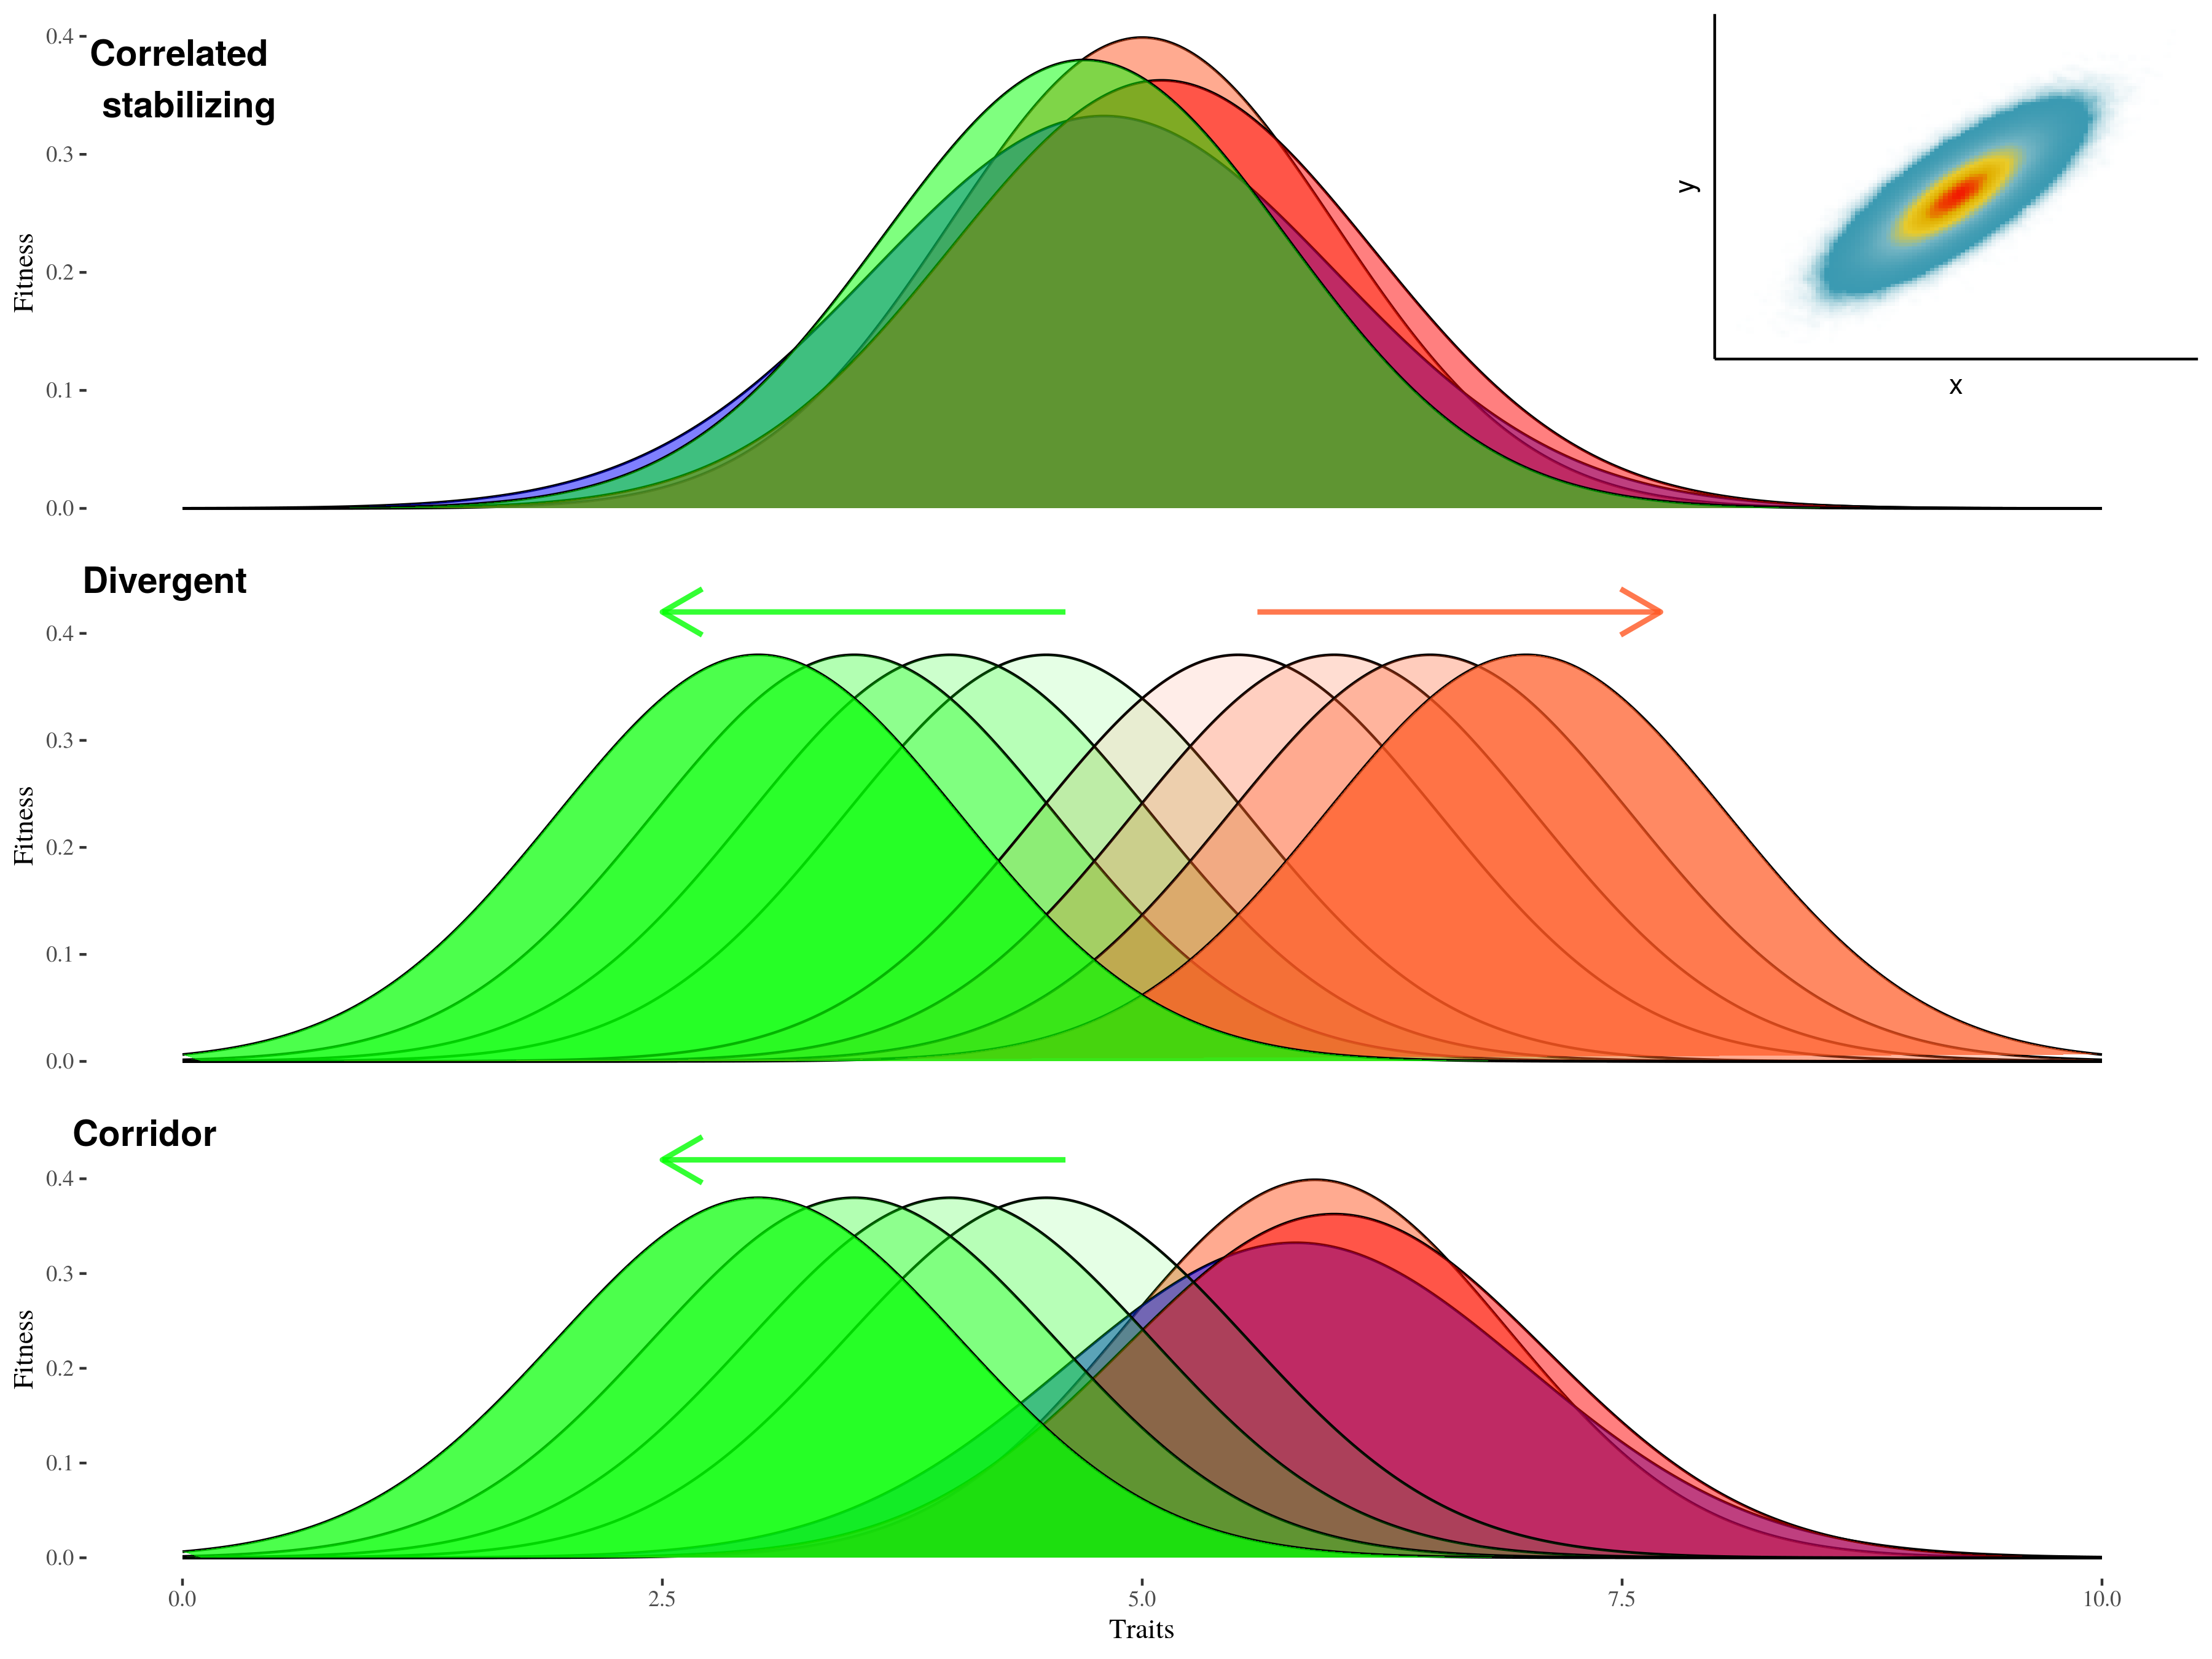
\includegraphics[width=\linewidth]{chapter_atchley/media/selection_types.png}
    \caption[Simulated selection regimes]{Representation of the simulated selection regimes. The Gaussian individual selection surface is defined by two parameters: the optimum and the selective surface covariance matrix. Under correlated stabilizing selection, the multivariate optimum for each trait is kept constant and the selective surface covariance matrix has non-zero off-diagonal elements that produce selection for positive correlations within modules, between traits [1,2] and [3,4] (upper right corner panel). Under divergent directional selection, the same correlated covariance surface is combined with a moving optimum. The optimum for traits [1, 2] is increasing, while the optimum for traits [3, 4] is decreasing. Under corridor selection, we again use the same correlation matrix, and the optimum for traits [1, 2] is increasing, while the optimum for traits [3, 4] is kept stationary.}
    \label{selectionregimes}
\end{figure}

\subsection{Mouse lines and phenotypes}

\subsubsection{Inbred strains} 
\label{ibs}

We founded an advanced intercross line using inbred strains derived from a
directional selection experiment by~\textcite{Atchley1997-vn}, in which each
strain was selected for increase or decrease in their early (0 to 10 days) and
late (28 to 56 days) growth rate, with corresponding compensatory selection in
the other direction. For example, the E+ selection strain corresponds to an
increase in early growth combined with a decrease in late growth. One of our
six strains had been selected for fast early growth (E+, A13 strain), two for
slow early growth (E-, A22 and A23 strains), one for fast late growth (L+, A31
strain), and two for slow late growth (L-, A41 and A42 strains). Before
selection, the additive genetic correlation between Early and Late growth in
the strain used the selection experiment was around 0.8. After selection, the
across selected strains genetic correlation between Early and Late growth was zero.
After the selection experiment, the strains were inbred for several
generations, and were all <1\% heterozygous. Unfortunately, during the several
years in which the selected strains were kept in an inbreeding regime, a
mistake in the labeling of the animals during a move for a new mice facility
led to a contamination of one of the E- strain (A22) with animals from one of
the L- (A42) and the other E- strain (A23). This contamination caused an
increase in the heterozigocity in the A22 line and some regions of the genome
where that are only five segregating haplotypes instead of the expected six.
We discuss this contamination further in the genotyping section.

\subsubsection{Breeding scheme}

The six inbred strains were crossed non-reciprocally in every pairwise
combination, giving 15 combinations in total. For three of the strains, 3
males and 2 females were used in crosses, each paired with a female or male
from one of the other strains. For the other three strains, the reverse was
true. This design gives an even balance of all six strains on the autosomes,
and close to an even balance of the strains on the Y-chromosome and the
mitochondria. From the F$_{\text{1}}$, two males and two females from each of
the 15 litters were used in mating pairs, giving 30 combinations in total. The
crossing scheme was designed such that there was no overlap in the strains
that had been crossed to produce the parents in the previous generation. That
is, each cross resulted in offspring that were a mixture of four of the
strains.  Furthermore, the two males from a given litter were mated to females
that themselves differed in both of the strains that had been combined to
produce them.  This maximized the number of different strain combinations, and
ensured representation of all six strains continued to be equal in the next
generation.  All crosses were reciprocal in this generation (i.e. if a male
from litter 1 was mated to a female from litter 2, then a male from litter 2
was mated to a female from litter 1).  A version of this design that balances
the contribution of each of the founder strains was continued up to the
F$_{\text{4}}$. However, each F$_{\text{2}}$ mouse was a mixture of four of
the six strains, therefore it was not possible to form pairs between unique
strain combinations in this generation.   To ensure all F$_{\text{3}}$ mice
included a contribution from all six strains, one male and one female from
each of the F$_{\text{2}}$ litters were used in non- reciprocal mating pairs,
again giving 30 (unique) combinations in total, but pairs were chosen such
that the parents overlapped in only two of the strains. This resulted in a
double dose of two strains in each F$_{\text{3}}$ offspring. To avoid unequal
distribution of the strains in the population, we ensured there was an equal
number of each pair of strains overlapping across the 30 pairs.  For the
F$_{\text{4}}$ generation, one male and one female from each of the
F$_{\text{3}}$ litters were used in mating pairs, again giving 30 combinations
in total. Each F$_{\text{3}}$ mouse was a combination of all six strains, with
a double dose of two strains. Pairs were chosen such that the male and female
did not overlap in the strains they had a double dose of (i.e. all
F$_{\text{4}}$ offspring ended up with a deficiency of two strains).  To avoid
unequal distribution of the strains in the population, we ensured there were
equal numbers of litters deficient in each pairwise combination of strains.
All crosses were non-reciprocal.  One pair failed to produce any offspring,
resulting in a very slight imbalance in the representation of the strains.
For generation F$_{\text{5}}$ and F$_{\text{6}}$, matting pairs were combined
at random, but avoiding within-litter mating and excluding duplicate litter
combinations. Two males and two females from each F$_{\text{4}}$ litter were
used in mating pairs, giving 58 combinations (due to one F$_{\text{3}}$ pair
failing to produce a litter). Finally, three males and three females from each
F$_{\text{5}}$ litter were used in mating pairs, giving 174 unique litter
combinations. On the day of birth, F$_{\text{6}}$ litters were trimmed to a
maximum of 10 pups (5 males, 5 females or as close to an even sex ratio as was
possible given the numbers born).  All litters were cross-fostered between
mothers within the breeding scheme within 2 days of birth (usually on the day
of birth, but occasionally later if a foster mother was not available).  Thus,
each female acted as a birth mother and a foster mother, and each litter was
reared by a different mother to the one that gave birth to it. In total, we
use 1513 animals from the F$_{\text{6}}$ generation.

\subsubsection{Phenotypes}

All mice were weighed on the day of birth, then at 3 days, 7 days and then
weekly until they were 8 weeks old. To define a low dimensional phenotype
related to growth, we used the difference in weight over 2 weeks. So our
analyses focus on weight gained over each two week interval (`growth') from
one week to eight weeks of age. These growth traits were calculated as the
difference in body weight between the weeks that define each time interval
(e.g., growth from birth to week 2 is defined as growth\textsubscript{0--2} =
weight\textsubscript{2} - weight\textsubscript{0}). The additive genetic
covariance matrix (G-matrix) between growth traits was estimated by an animal
model in ASReml-R v3~\parencite{ASReml} using the phenotypes of the
F$_{\text{5}}$ and F$_{\text{6}}$ generation and the population pedigree. Sex
was included as a fixed effect.
  
\subsubsection{Genotypes}

The genomic data was extracted from the spleens of one mouse for each of the
inbred strains. Each strain was then run in each lane of a flow cell and
sequencing was conducted using paired end Illumina sequencing. This produced
approximately 487 million total bases for each sample, all of 125bp in length.
Galaxy~\parencite{Goecks2010-hz} was used to conduct quantity control using
FastQC on the untrimmed sequences. The sequence reads were trimmed in
trimmomatic~\parencite{Bolger2014-ra} using the following parameters: Cropped
first 10 bases from each read, trimmed specified adapter sequences, allowed a
maximum of 2 mismatches between the adapter and read sequence, palindrome Clip
Threshold of 30, simple Clip Threshold of 10, minimum length of adapter
detected of 8 bases, and retaining the reverse read to maintain pairing
(\texttt{keepBothReads=true}). Following the trimming, we removed leading and
trailing bases from reads with quality less than 3 using a sliding window of 4
bases and trimmed if mean quality was less than 15. The trimmed transcripts
were then paired and aligned to mouse reference genome (mm10) using Bowtie 2
\parencite{Langmead2012-ev}. The \texttt{‘Local, sensitive’} alignment
algorithm was used, with all other parameters left unchanged. After alignment,
SNP calling was carried out using SAMtools~\parencite{Li2009-yr} against the
mm10 reference genome. The tool \texttt{‘Pileup’} was used to identify SNPs,
with  parameters set to default. From this set of SNPs we set out to design a
custom SNP array for genotyping in the intercross generations. Our initial
strategy for designing the SNP genotyping array was to select private SNPs for
all the strains along the genome. Private SNPs are SNPs that are biallelic
among the founder strains, with one strain having one allele and the other
five strains sharing the alternate allele. If the density of private alleles
is high enough, this provides a trivial way of identifying the strain of
origin of a particular stretch of the genome in the intercross line. However,
the labeling mistakes in the maintenance of the inbred strains (described in
section~\ref{ibs}-\textbf{Inbred Strains}) caused some degree of interbreeding
between some of the strains. This made selecting the SNPs for the genotyping
array a more challenging task, since in some regions of the genome some of the
strains lacked private alleles that would lead to the most informative SNP
choice. Given this problem, we developed piecewise approach to select, in each
segment of the genome, the most informative set of SNPs available. We divided
the full genome into equal sized chunks, and in each chunk ranked the SNPs in
terms of their information content: first private alleles (5:1 split of the
strains), then SNPs where one allele was shared between two of the strains
(4:2 splits) and finally SNPs where one allele was shared between three of the
strains and the other between the other three strains (3:3 splits). We
classified the SNPs into these broad groups, and then classified them into
categories using the strains involved in the splits, so, we have 6 types of
5:1 SNPs, 15 types of 4:2 splits, and 10 types of 3:3 splits. We then selected
at most 4 SNPs for each of these 31 classes of SNPs, totaling at most 50 SNPs
per chunk. Selection for the SNPs in the same class was done by selecting the
most high quality SNPs (as ranked by SAMtools). This resulted in a set of
around 50000 SNPs with maximal information for each chunk that were used by
Affymetrix to produce a custom SNP array\footnote{Fast parallel code for
performing this SNP selection can be found in \url{https://github.com/diogro
/EL-snp_selection}}. Using this array, we scored 55338 SNPs, of which 43934
were polymorphic in the intercross. These SNPs were scored in 2299 samples
divided among the inbred parental strains, the F$_{\text{1}}$, F$_{\text{5}}$
and F$_{\text{6}}$ generation. Quality control was done using the Affymetrix´s
\textsc{Axiom Genotyping Solution: Data Analysis
Guide}\footnote{\url{https://tools.thermofisher.com/co
ntent/sfs/manuals/axiom_genotyping_solution_analysis_guide.pdf}, last viewed
in September 20th, 2018}. Samples with call rate below 97\% were discarded,
resulting in 2243 samples. SNP quality control was done using Axiom Analysis
Suite\footnote{\url{https://www.thermofisher.com/us/en/home/life-science
/microarray-analysis/microarray-analysis-instruments-software-services
/microarray-analysis-software/axiom-analysis-suite.html}, last viewed in
September 20th, 2018}, and after standard quality control filtering we arrived
at a final set of 33300 high quality biallelic SNPs distributed along the
genome. These SNPs were scored in 1513 individuals from the F$_{\text{6}}$
generation, 629 from the F$_{\text{5}}$, 50 from the F$_{\text{1}}$, e 26
parental individuals from the inbred strains. Phasing and imputation of
missing SNP calls was done in Beagle 4.0 \parencite{Browning2007-el}, using
the parent-offspring relations among the individuals to inform the imputation.

\subsection{QTL mapping}

In order to link genetic and phenotypic variation, QTL mapping was performed
in the F$_{\text{6}}$ generation of the intercross using a multivariate mixed model
implemented in GEMMA v0.97~\parencite{Zhou2014-op}. The inclusion of a random
effect is necessary to take the relatedness of the individuals in the F$_{\text{6}}$ into
account. We estimate the relatedness matrix using the full set of SNPs in
GEMMA with a leave-one-chromosome-out approach~\parencite{Yang2014-hl}. In
this approach, when fitting the model to a given SNP, we exclude the
chromosome containing the focal SNP from the relatedness calculation. This
method increases power to detect genotype phenotype associations as the signal
from the focal SNP is not masked by the relatedness. GEMMA estimates an
additive effect vector of each SNP on the growth phenotypes, and the
significance of each of these fixed effects is assessed using a Wald test. As
the SNP are correlated, we use the GEC software provided
by~\textcite{Li2012-wl} to calculate the effective number of markers in each
chromosome, and, using a Bonferroni correction, establish a per-chromosome
significance threshold corrected for multiple tests. We filter all the
significant SNPs at the per-chromosome thresholds, and if two or more
significant SNPs in the same chromosome are closer than 20cM we select only
the most significant SNP in that interval. We also calculate a genome-wise
significance threshold that provides additional confidence to some SNPs, but
we do not use this threshold in selecting the markers. We then analyze the
additive effects of the identified significant SNPs on the multivariate growth
traits.

\subsection{Genetic effects and covariation}

In both the simulations and the QTL mapping we have pleiotropic effect vectors
that describe the effect of an allele on a set of traits. The pattern of
pleiotropy will largely determine the genetic covariation we observe between
traits (see Chapter 5). Alleles that increase two traits simultaneously will
contribute to the positive correlation between these traits, while alleles
that affect traits in different direction will contribute to the negative
correlation between the traits. If two traits don't share genetic effects, the
contribution of pleiotropy to the correlation between them is zero, and any
genetic correlation we observe will be due to linkage or non-additive genetic
effects. Working with a known or putative modular partition of the traits, we
can classify these genetic effects on multiple traits by the sign of the
effects on each of the traits in relation to the modularity hypothesis. For
example, an allele that only increases two traits in the same module is
defined as modular, while one effect that increases the traits in one module
while decreasing the traits in a different module is antagonistic.  We give
some examples for four traits in Fig.~\ref{effectclassification}, assuming
traits [1,2] and [3,4] form modules. When classifying the alleles in the
simulations, we first calculate the mean allelic effect at each loci by taking
the average of all the alleles at a given loci. Then, we classify these mean
pleiotropic vectors in the simulations and the estimated vectors of QTL
effects according to their vector alignment with the directions shown in
Fig.~\ref{effectclassification}, i.e. a vector is classified according to the
direction it is most aligned with. In the QTL analysis,  we use these effect
vectors to estimate the additive genetic  covariance matrix directly from all
the QTLs using the equations from Chapter 5, and we also estimate the expected
covariance matrix from the QTLs classified into a given class.


\begin{figure}
    \centering
    \subfloat[Effect classes]{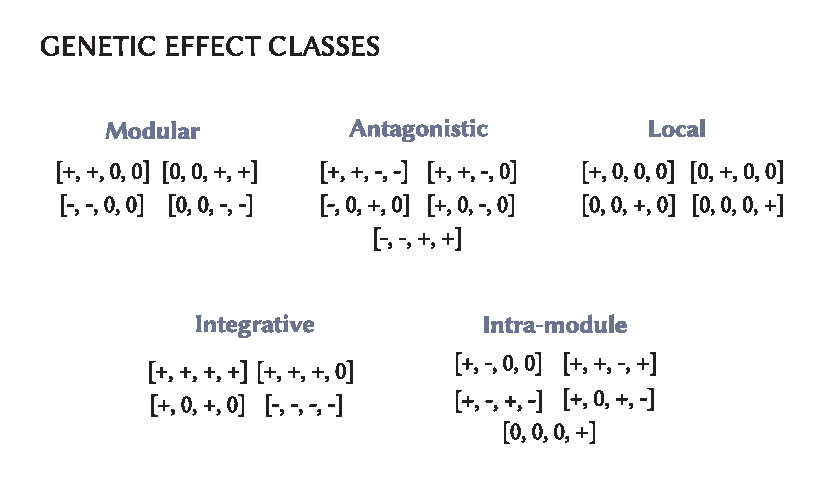
\includegraphics[width=\linewidth]{chapter_atchley/media/genetic_effects.eps}} \\
    \subfloat[Two dimensional classification boundaries]{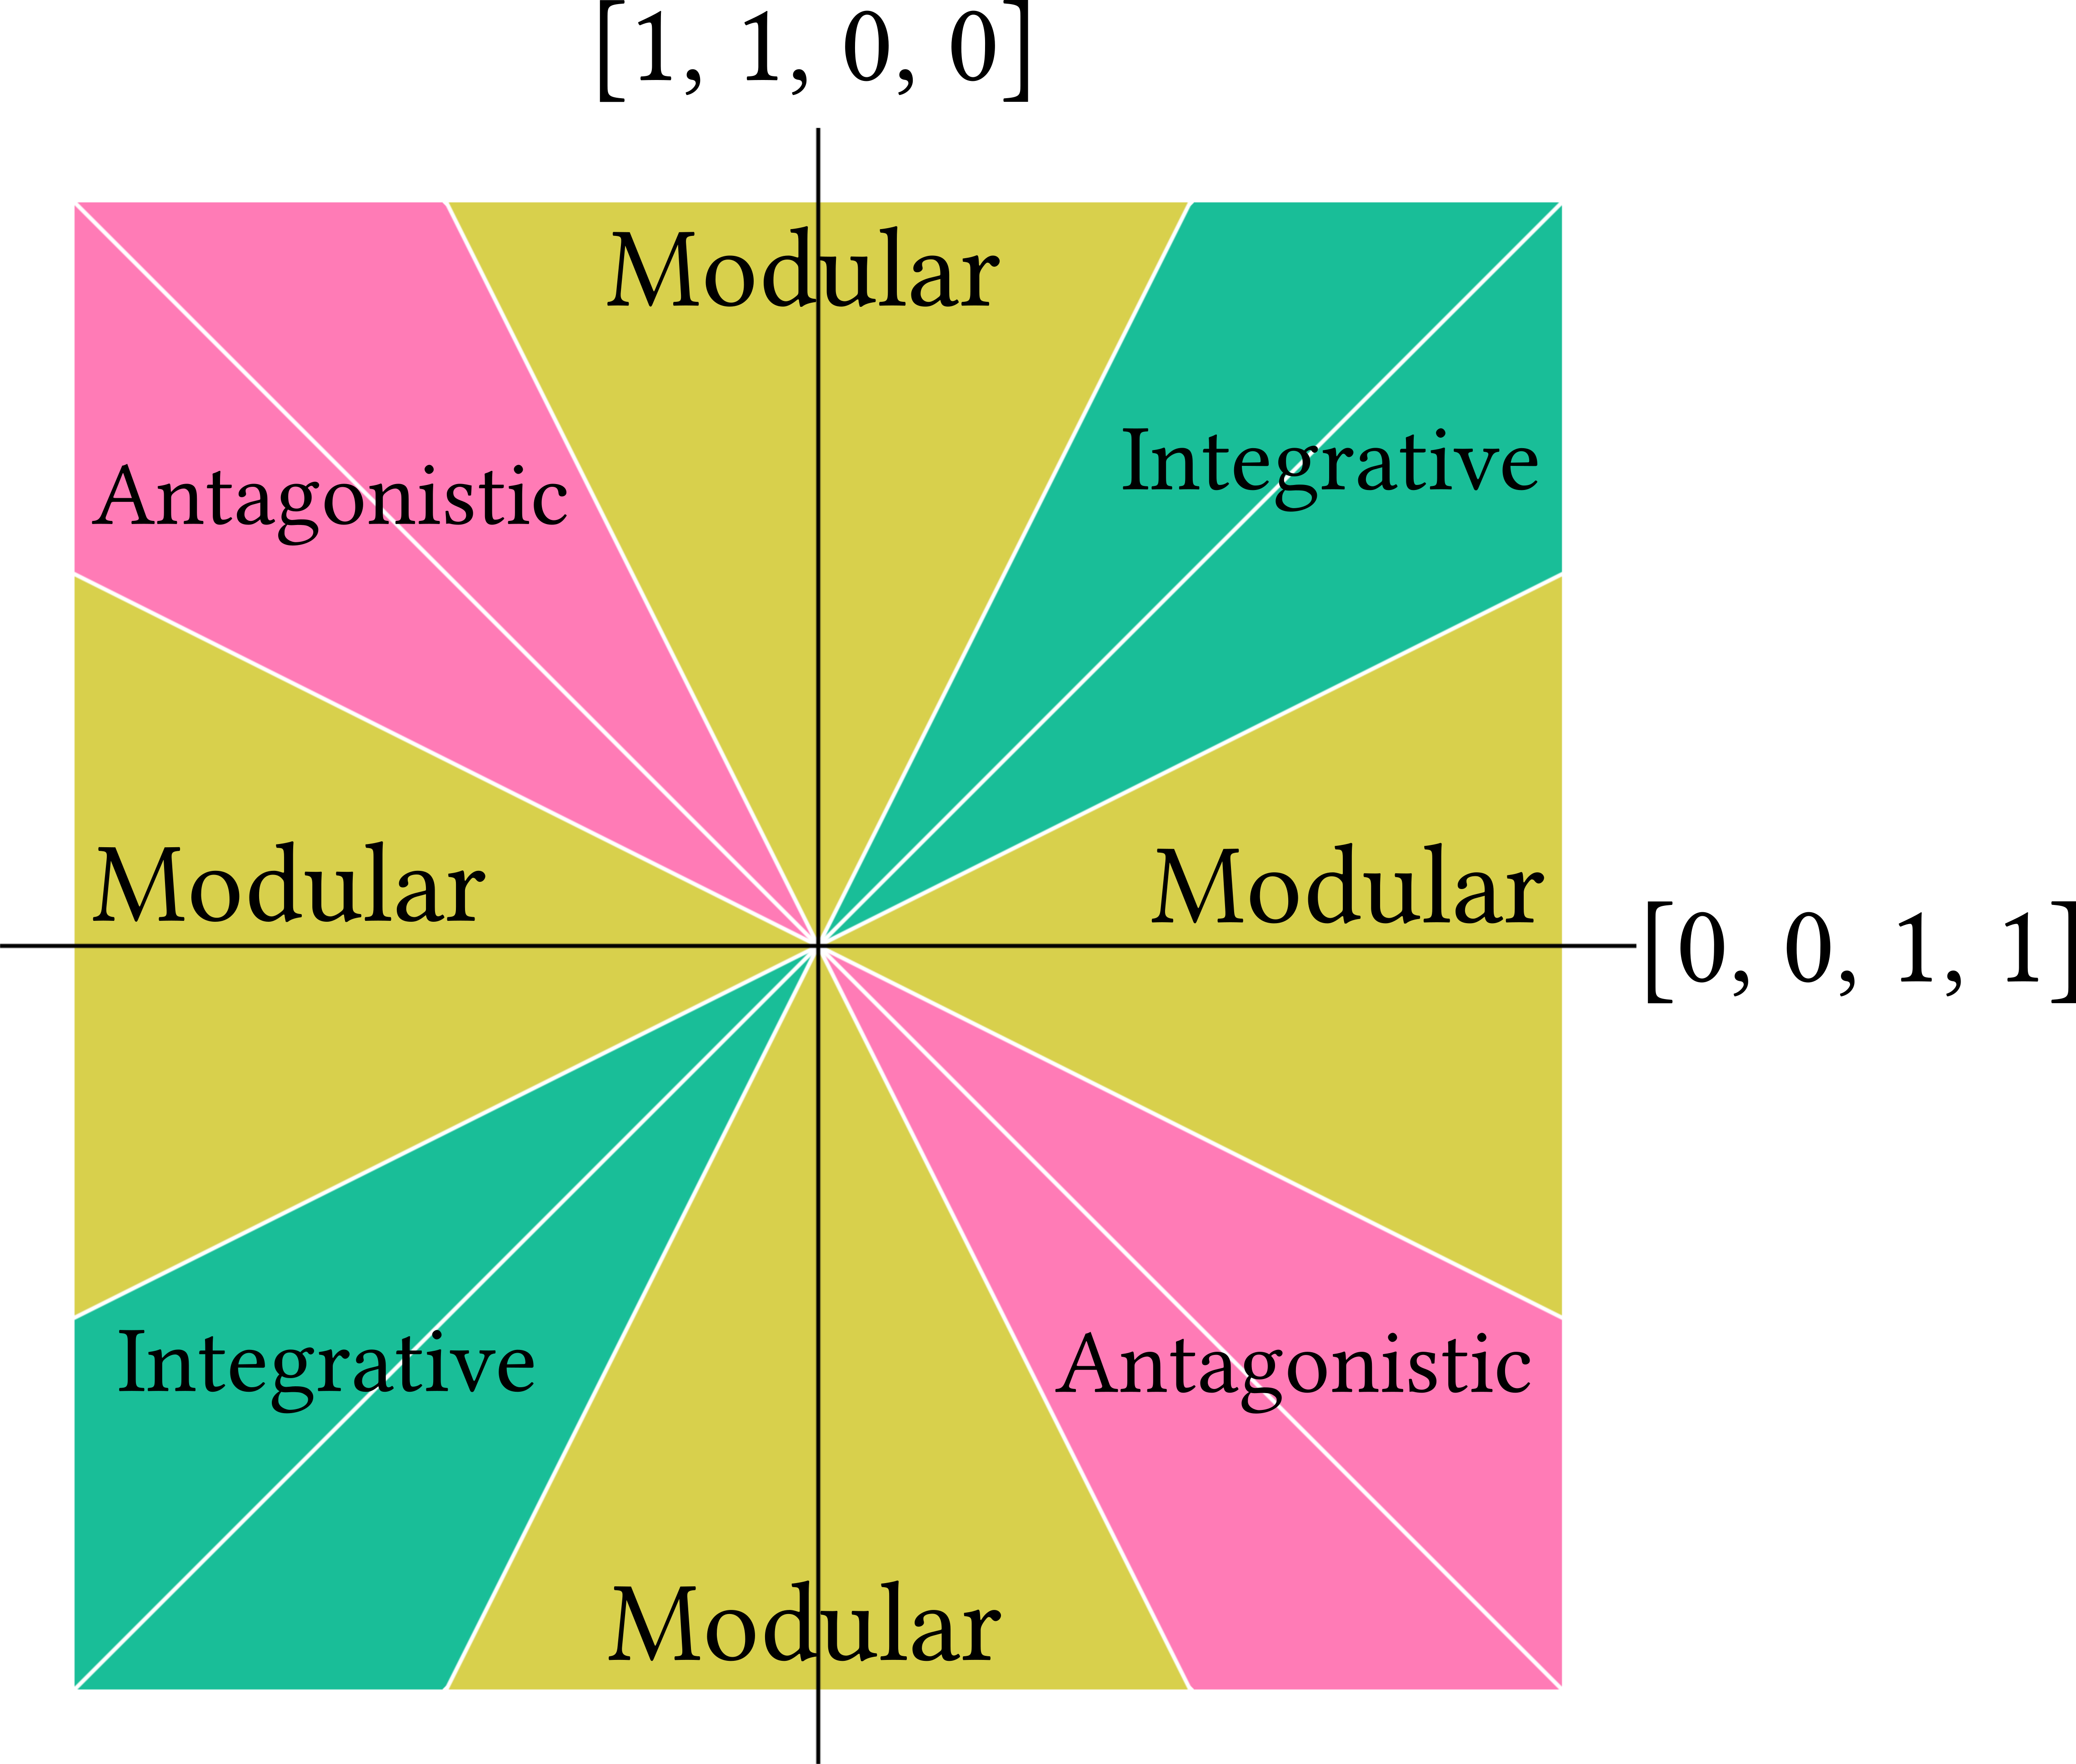
\includegraphics[width=250px]{chapter_atchley/media/vector_classifcation_fig.png}}
    \caption[Pleiotropic vector classification]{a) Pleiotropic genetic effect can be classified according to the direction of the effect on multiple traits with regards to a modularity hypothesis. For example, modular allelic effects can be defined as those that change two or more traits in a module in the same direction, while having no effect in traits outside that module. We also define antagonistic effects as those that have effects in two or more modules in opposite directions, i.e. increasing module 1 while decreasing module 2. Local effects affect only one trait, integrative effects affect two of more modules in the same direction, and finally intra-module effects affect traits in opposite directions inside the proposed modular structure. A non-comprehensive set of examples is shown in panel a) assuming a four trait two module. b) The decision boundaries in the two dimensional plane composed of the two-module directions. Effects along the axis (modules) are modular, effects along the main diagonal are integrative and effects along the secondary diagonal are antagonistic. Intra-modular and local effects do not appear in this plane.}
    \label{effectclassification}
\end{figure}


\section{Results}

\subsection{Simulations}


All simulated population responded to the selective regimes. The population
under stabilizing selection was kept at the optimum for all traits and showed
a two-module covariation pattern compatible with the correlated selection.
Both populations under directional selection tracked the optimum closely,
changing their mean phenotypes in response to selection
(Fig~\ref{simulated:t1}). All selection regimes lead to modular covariation
matrices, with higher correlations within modules than between modules
(Fig.\ref{simulated:t2}), however, differences between the selection regimes
appear when we examine the pattern of pleiotropy. Stabilizing selection leads
to a large proportion of local and intra-module effects, which do not
contribute to the observed two module pattern. Modularity under stabilizing
selection is due to a combination of a small number of modular effects and a
larger number of antagonistic and integrative effects. Under directional
selection, there is a large increase in allelic effects aligned with
selection, while still maintaining variational modularity. Under divergent
selection, most effects are antagonistic, while under corridor selection many
effects are modular, but we still see integrated and antagonistic effects.
Fig.~\ref{simulated:t3} shows the number of effects in each class for all
selection regimes. 

\begin{figure}[htbp]
    \centering
    \subfloat[Mean phenotypes.]{\label{simulated:t1}\includegraphics[width=200pt]{fsm}}\vspace{20pt}
    \subfloat[Genetic correlations.]{\label{simulated:t2}\includegraphics[width=200pt]{fsm}}\\
    \vspace{-18pt}
    \subfloat[Mean allelic effects classification.]{\label{simulated:t3}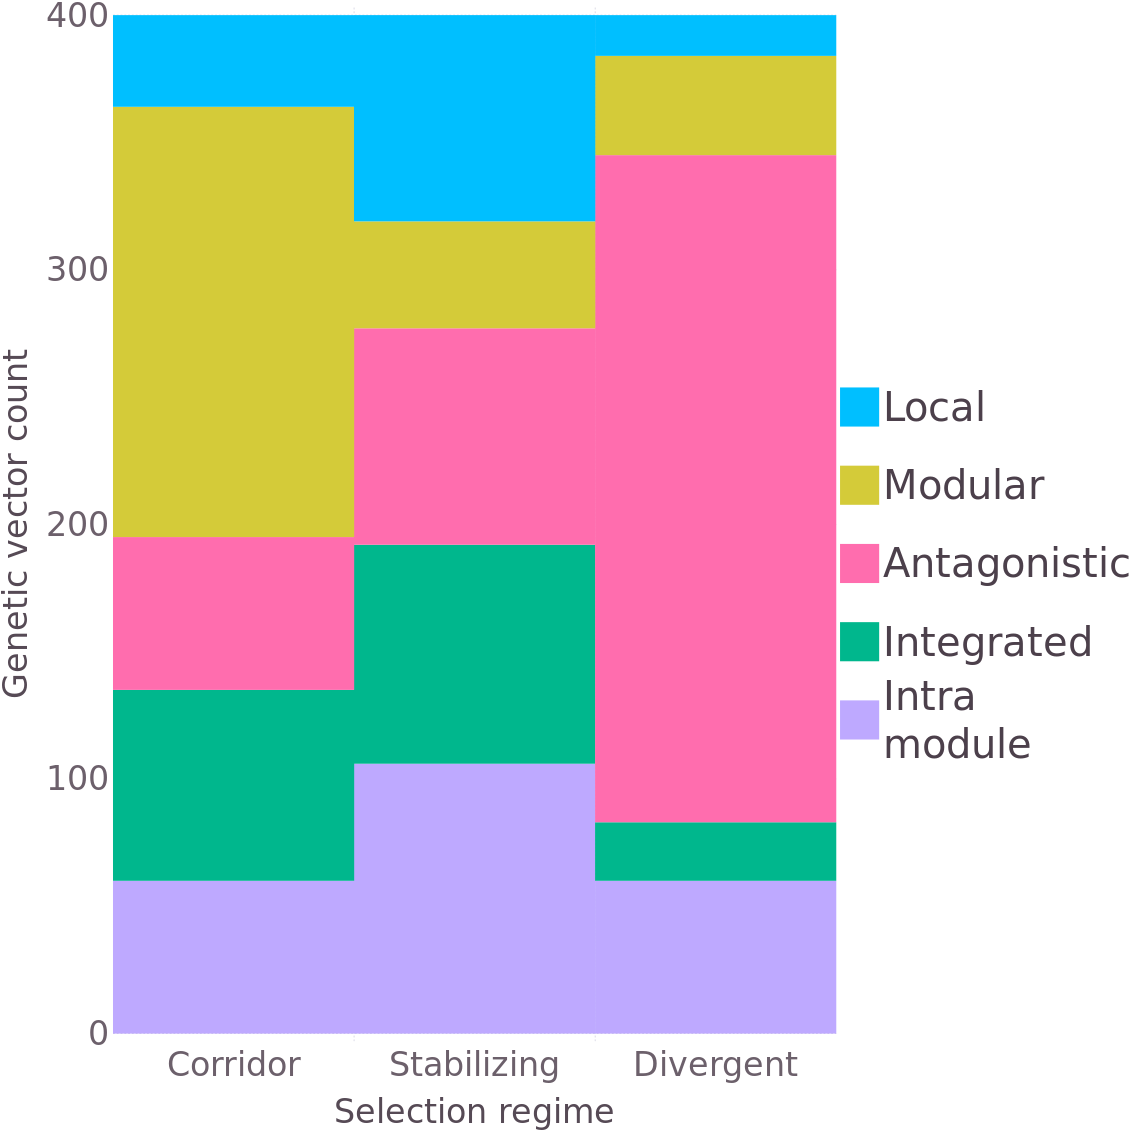
\includegraphics[width=300pt]{chapter_atchley/media/genetic_effect_classes_simulations}}\vspace{11pt}
    \caption[Simulation results]{Simulation results. a) Changes in the selective surface optimum and corresponding changes in mean phenotypes for the populations under directional selection. b) Genetic correlation matrices for simulated populations. c) }
    \label{simulated}
\end{figure}

\subsection{Advanced intercross line}

\subsubsection{Phenotypes}

Mean growth phenotypes measured in the inbreed founder lines and for all
individuals in the F$_{\text{6}}$ are shown in Fig.~\ref{growthcurves:t1}. The
F$_{\text{6}}$ population has more variation in growth than the between line
differences, suggesting that interactions and environmental effects are
present in the F$_{\text{6}}$ variation, along with the expected additive
variation. One noteworthy difference between the overall distribution of the
founders and the F$_{\text{6}}$ is that in the founder three of the six
strains have a maximum of growth in the second two week period, while the
other three strains have the maximum at the third interval, while in the
F$_{\text{6}}$ most individuals have a peak in the second interval, suggesting
some dominance between strains. Also, in the first two periods, the mean for
the F$_{\text{6}}$ is above the mean for the founders, suggesting that
environmental or maternal effects are present. The additive genetic
correlation matrix in the F$_{\text{6}}$ is organized in the familiar two
module pattern for early and late growth (as in Chapter 5). We see positive
correlations between two traits in each of the two periods, and negative or
null correlations between the two phases (Fig.~\ref{growthcurves:t2}). In the
ancestral strain used in the selection experiment that produced our founder
inbreed strains the correlation between Early and Late growth was positive, so
the negative and null correlation we see across the inbreed lines and in the
F$_{\text{6}}$ are a result changes in genetic architecture due to divergent
directional selection~\parencite{Atchley1997-vn}. The negative correlation
between the first late interval and the early intervals is strictly speaking
not compatible with a modular architecture as there is a dependency between
the two phases. In spite of this, we still use this putative modular structure
since it is compatible with the pattern of positive correlations and congruent
with the artificial selective experiment.

\begin{figure}
    \centering
    \subfloat[Inbreed strains and F$_{\text{6}}$ generation growth phenotypes.]{\label{growthcurves:t1}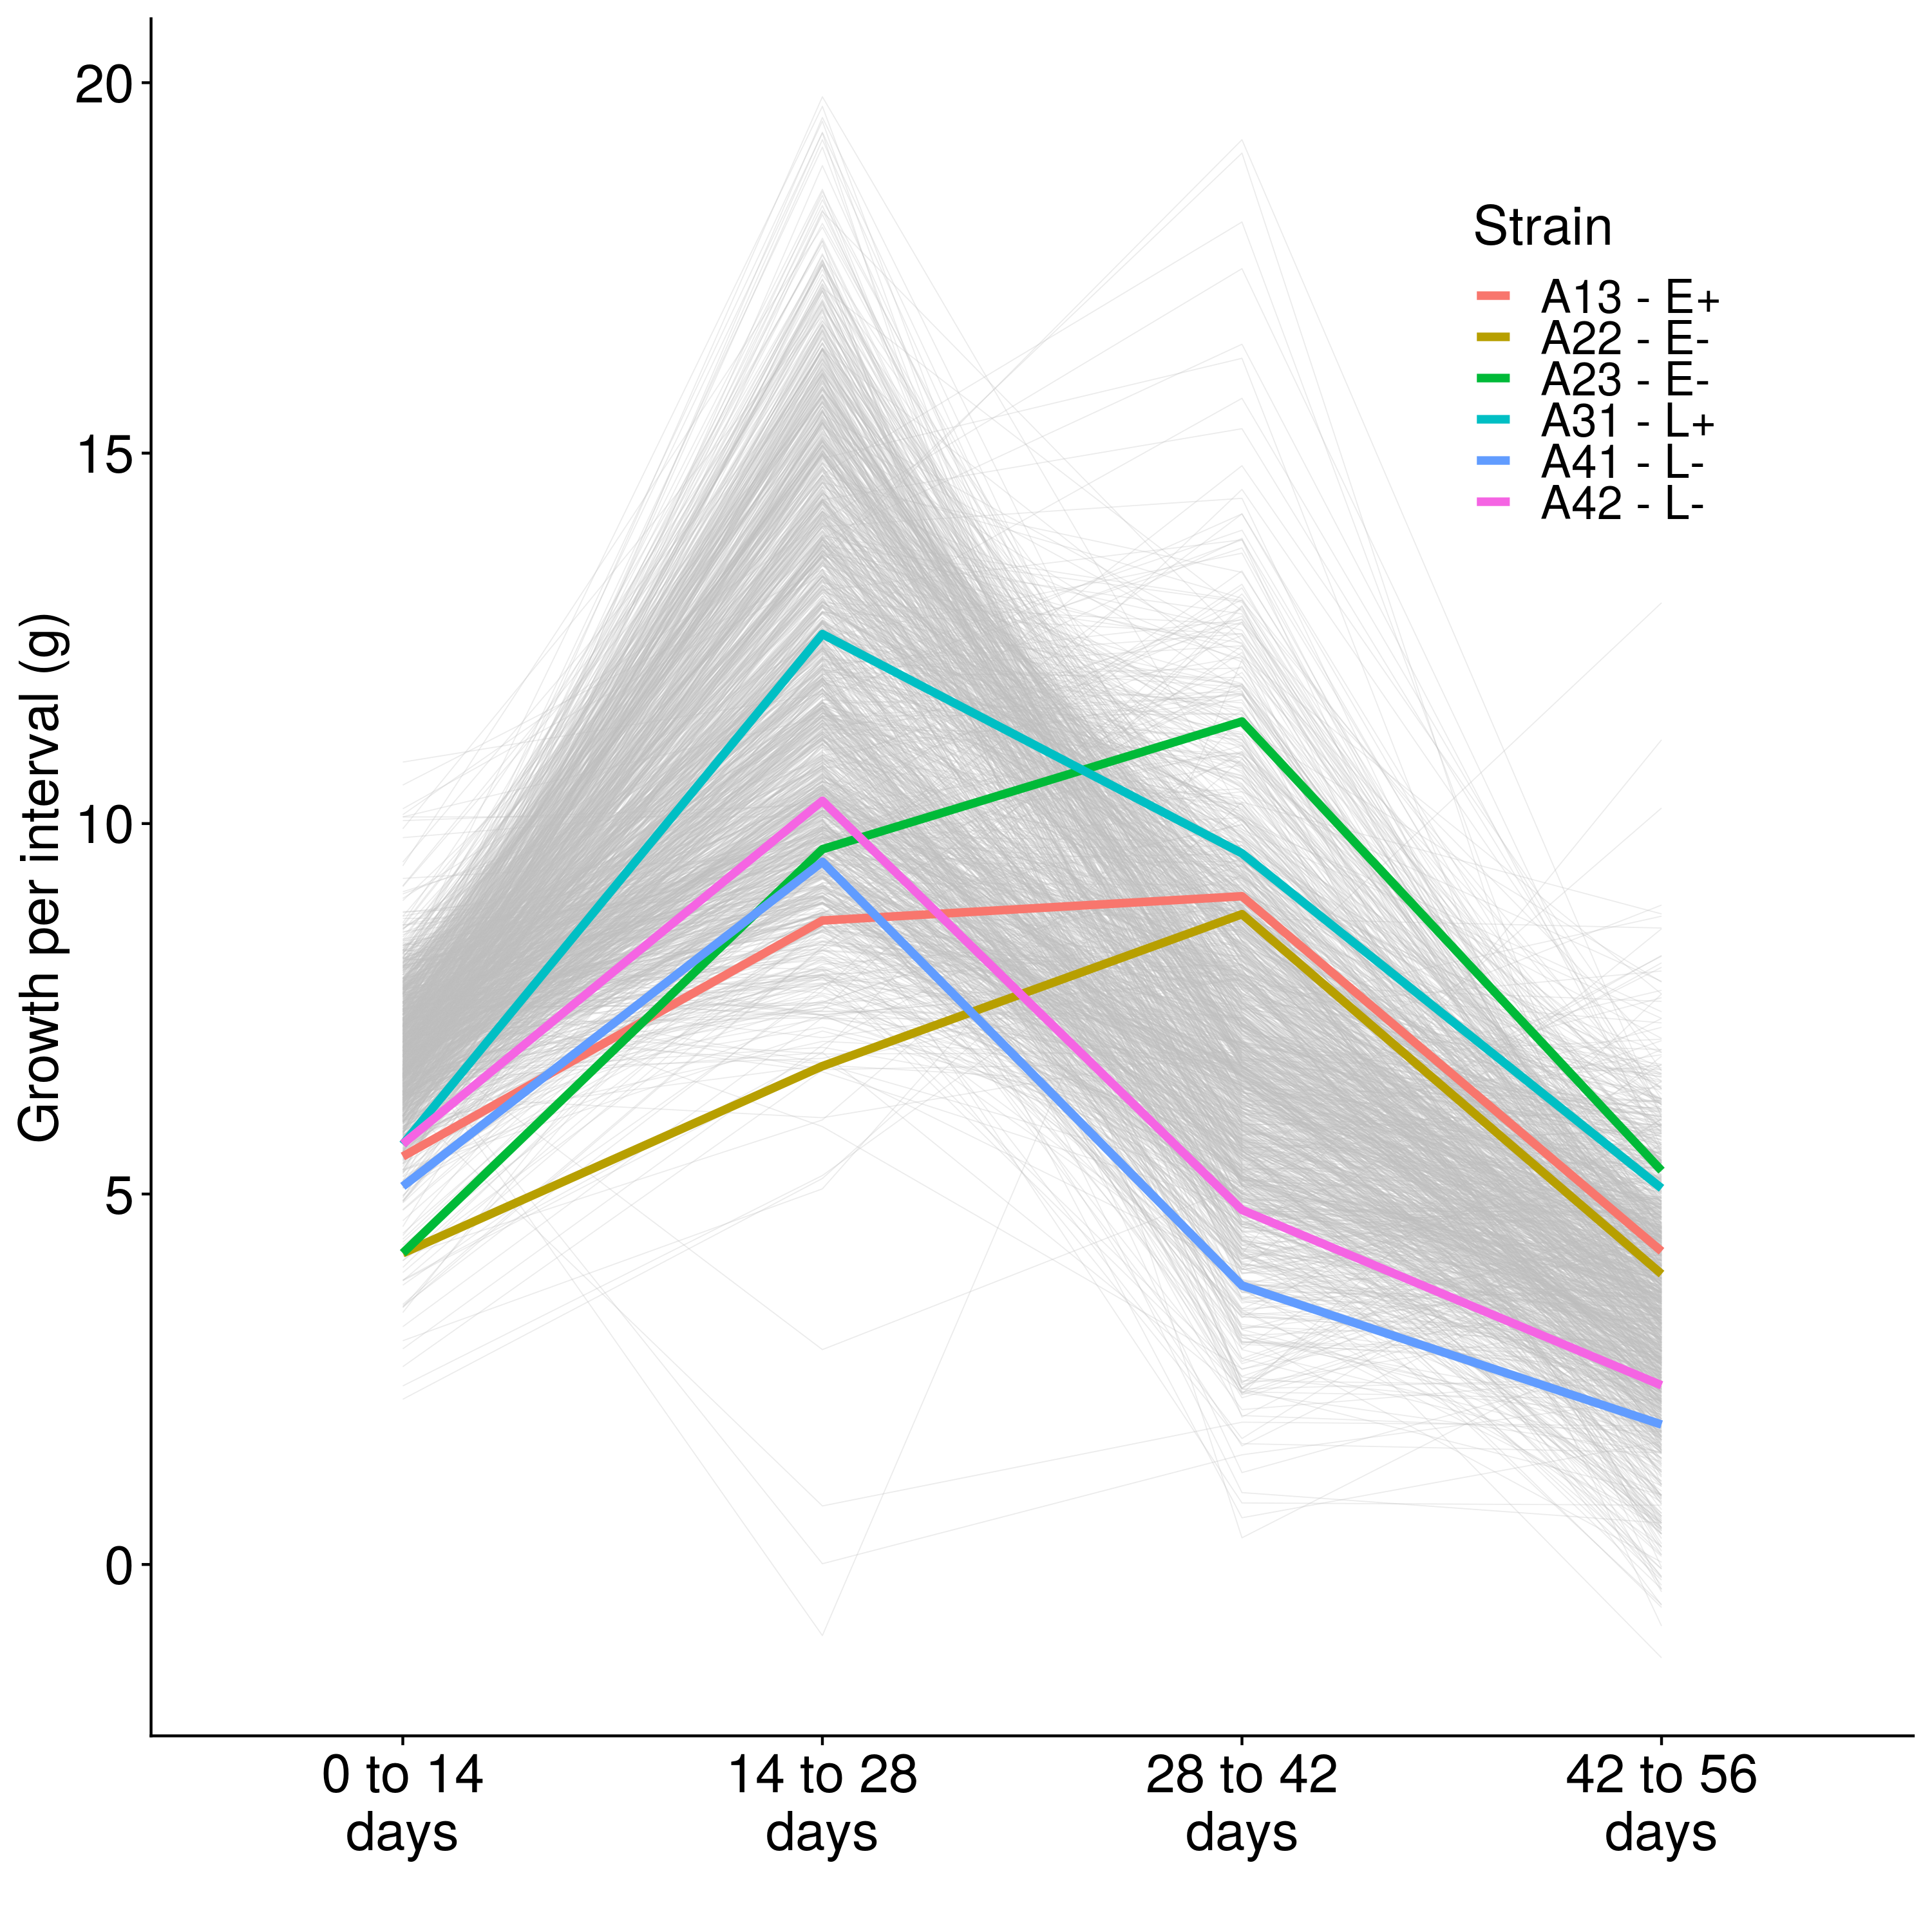
\includegraphics[width=300pt]{chapter_atchley/media/strain_growth-curves_2w}} \\
    \subfloat[Additive genetic correlation for growth traits.]{\label{growthcurves:t2}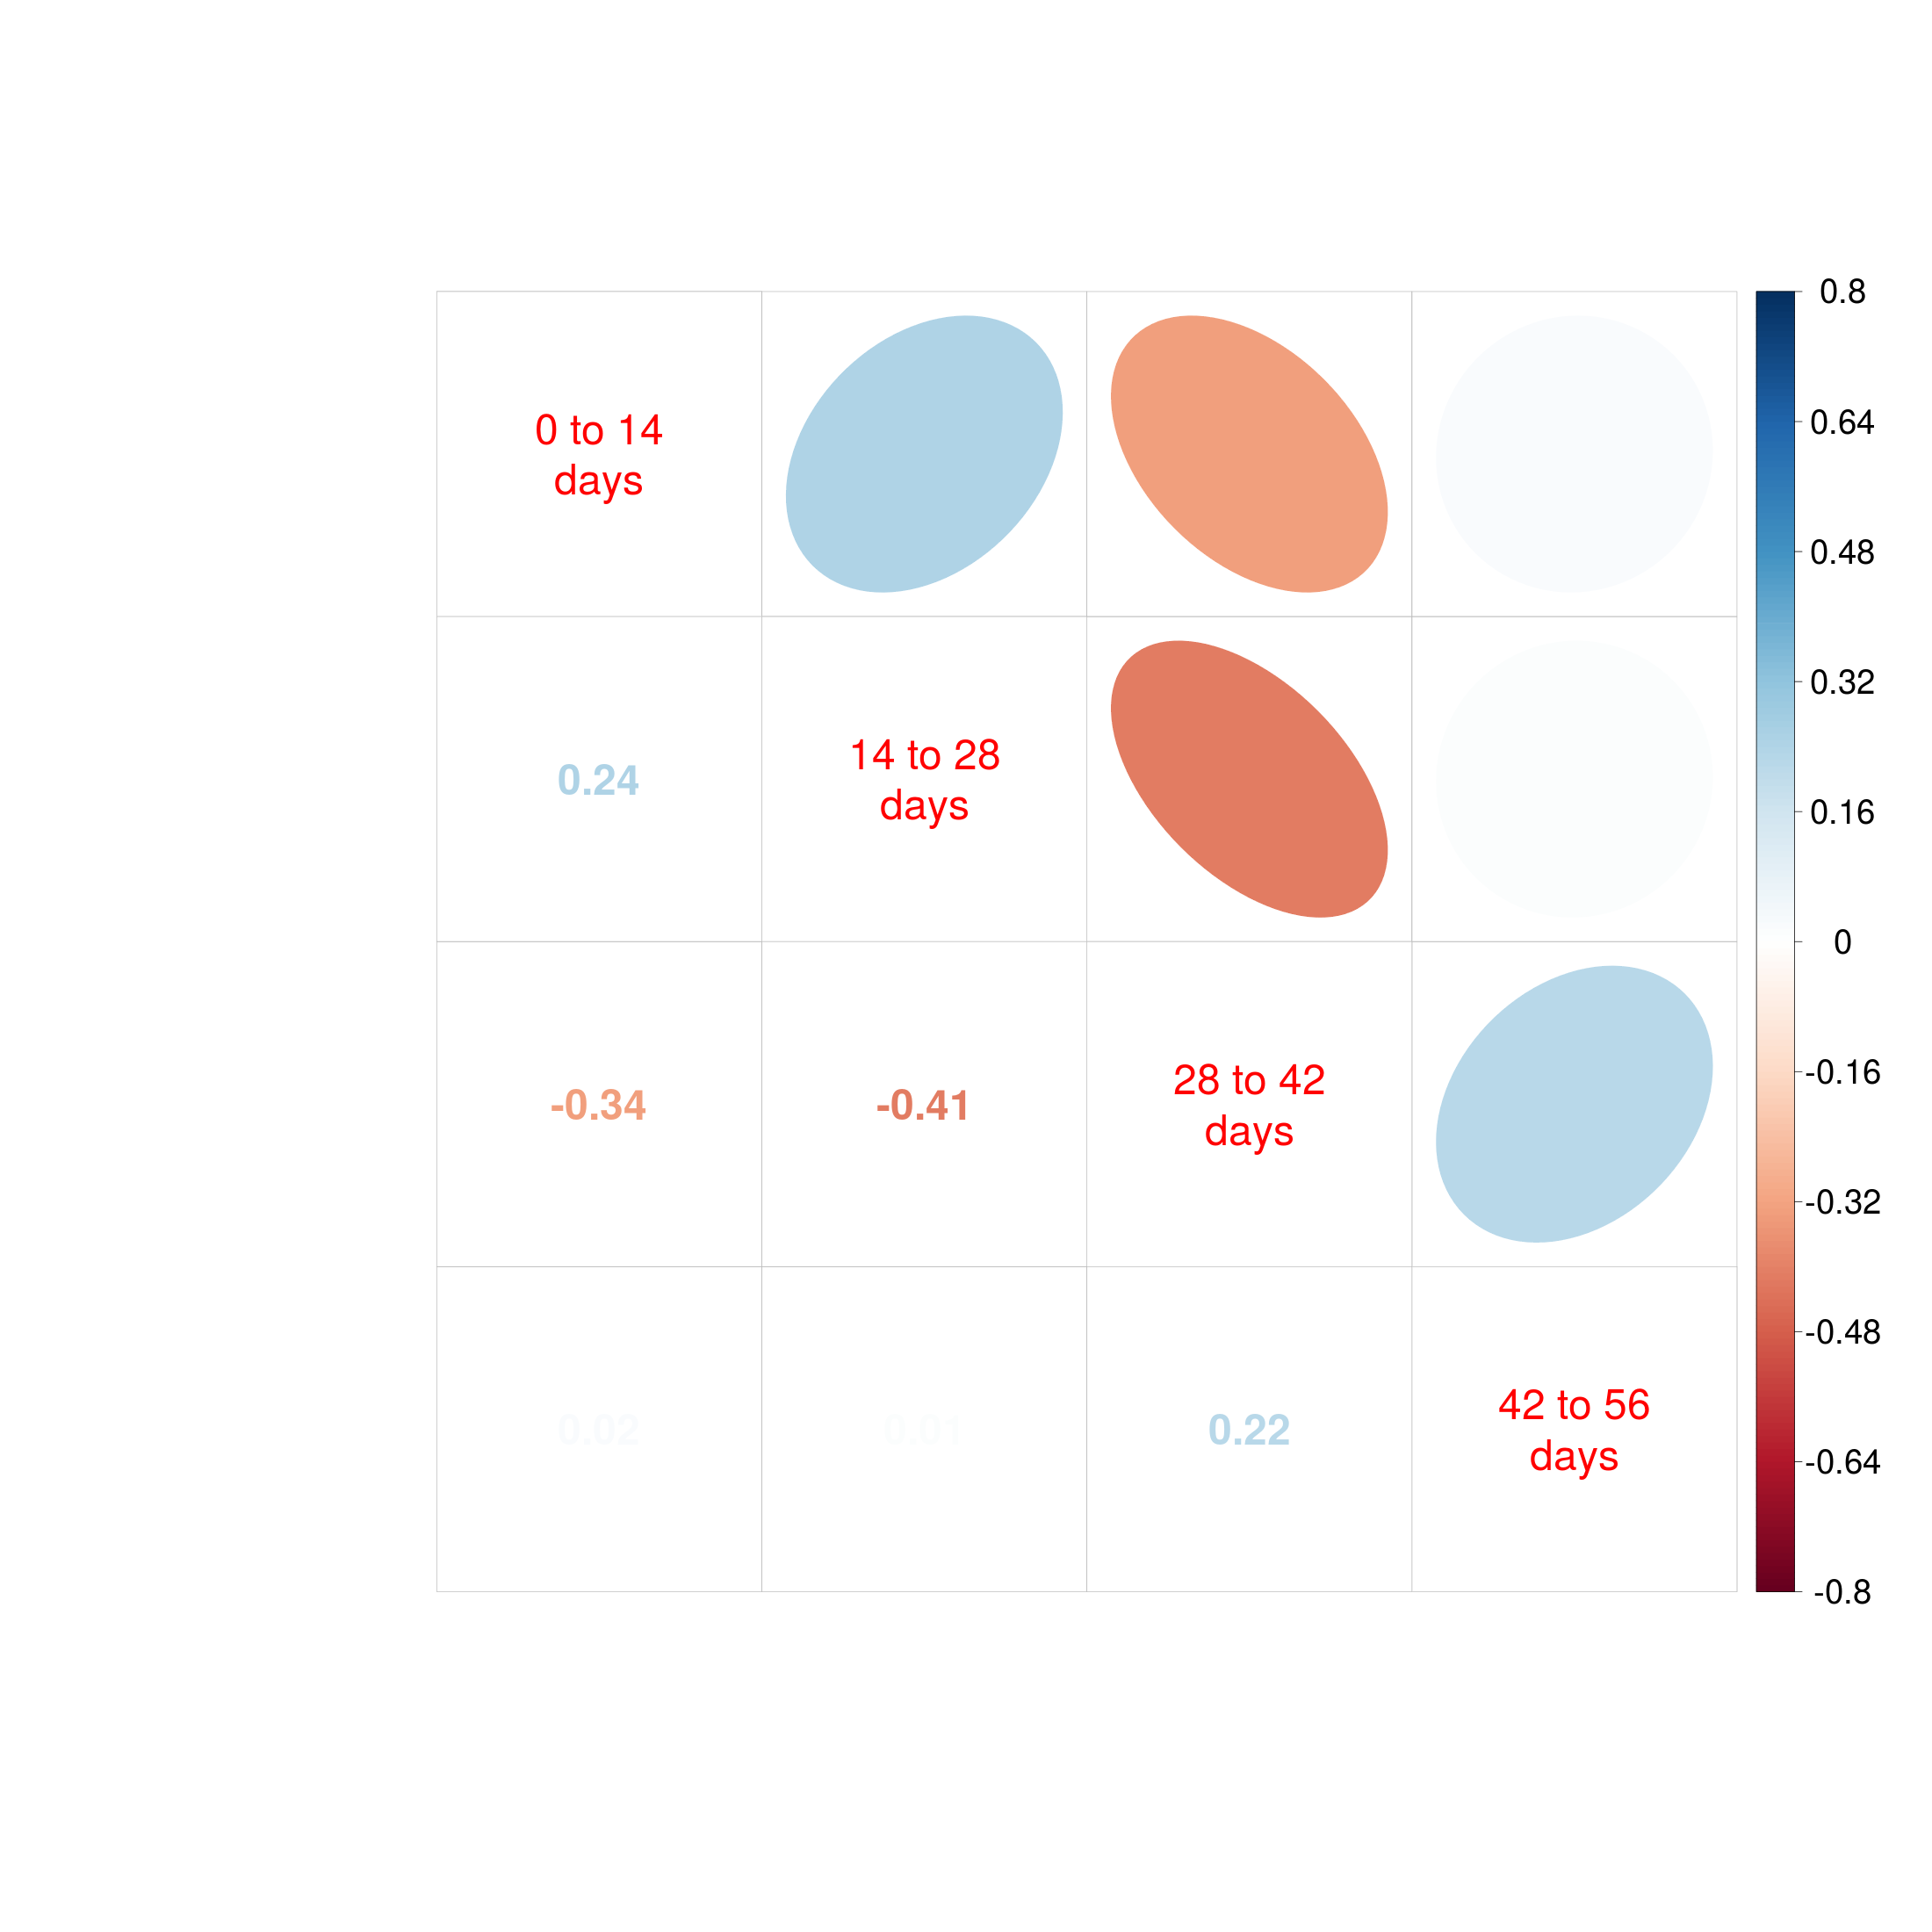
\includegraphics[width=300pt]{chapter_atchley/media/growth_Gmatrix_2w_4t.png}}\\
    \caption[F$_{\text{6}}$ growth phenotypes]{Growth phenotypes of the inbreed founders in color and the full F$_{\text{6}}$ population in thin gray lines.}
\end{figure}

\subsubsection{QTL effects}

We detected 33 pleiotropic QTLs at the per-chromosome 5\% significance level,
of which 15 were also significant at the 5\% genome-wide level
(Fig.~\ref{manhattan}, Table~\ref{qtltable}). These QTLs were classified using
their directions in trait space according to a putative Early-Late modular
hypothesis\footnote{We point out that while the Early-Late hypothesis is
reasonable and common in growth studies, it is not completely supported by
F$_{\text{6}}$ covariance matrix due to the negative dependency between Early
and Late intervals. We continue to use this hypothesis because it is supported
by the within-module correlations and is congruent with the selection regimes
the inbreed founders are derived from, and so is expected to structure the
variation in the F$_{\text{6}}$.}. All effects vector classes were represented
in the detected QTLs: 6 modular, 1 local, 11 intra-module, 7 integrated, 8
antagonistic. We use these effect vectors to estimate the expected covariance
matrix from all the QTLs and for the QTLs in each genetic effect class. The
full QTL additive matrix, using all detected QTL effects, captures the overall
pattern of additive genetic correlations, but the non-null correlations are
lower than the ones observed in the G matrix. Within growth period
correlations are positive and larger than the between module correlations. The
only difference in pattern is that the correlations between the first interval
and the the third interval is negative in the G-matrix and positive in the QTL
matrix. The other negative correlation, between intervals 2 and 3 is present
in both. When we examine the matrix estimated from the QTLs separated into
classes we don't see a clear picture. Most of the modular effects are
concentrated in the Late traits, and accordingly we see large correlations
involving these traits in the modular effects QTL matrix. We do not see a
clear modular pattern in the matrix estimated from the modular effects. The
intra-module effects produce negative correlations between the third interval
and the Early traits. We would expect the integrated effects to produce
positive correlations, but we still see two cases of negative correlations.
The antagonistic effects also defy our expectation, as they are expected to
produce positive within module correlations and negative between module
correlations. Instead, we see mostly positive correlations and a single
negative correlation between intervals 1 and 3.


\begin{figure}
    \centering
    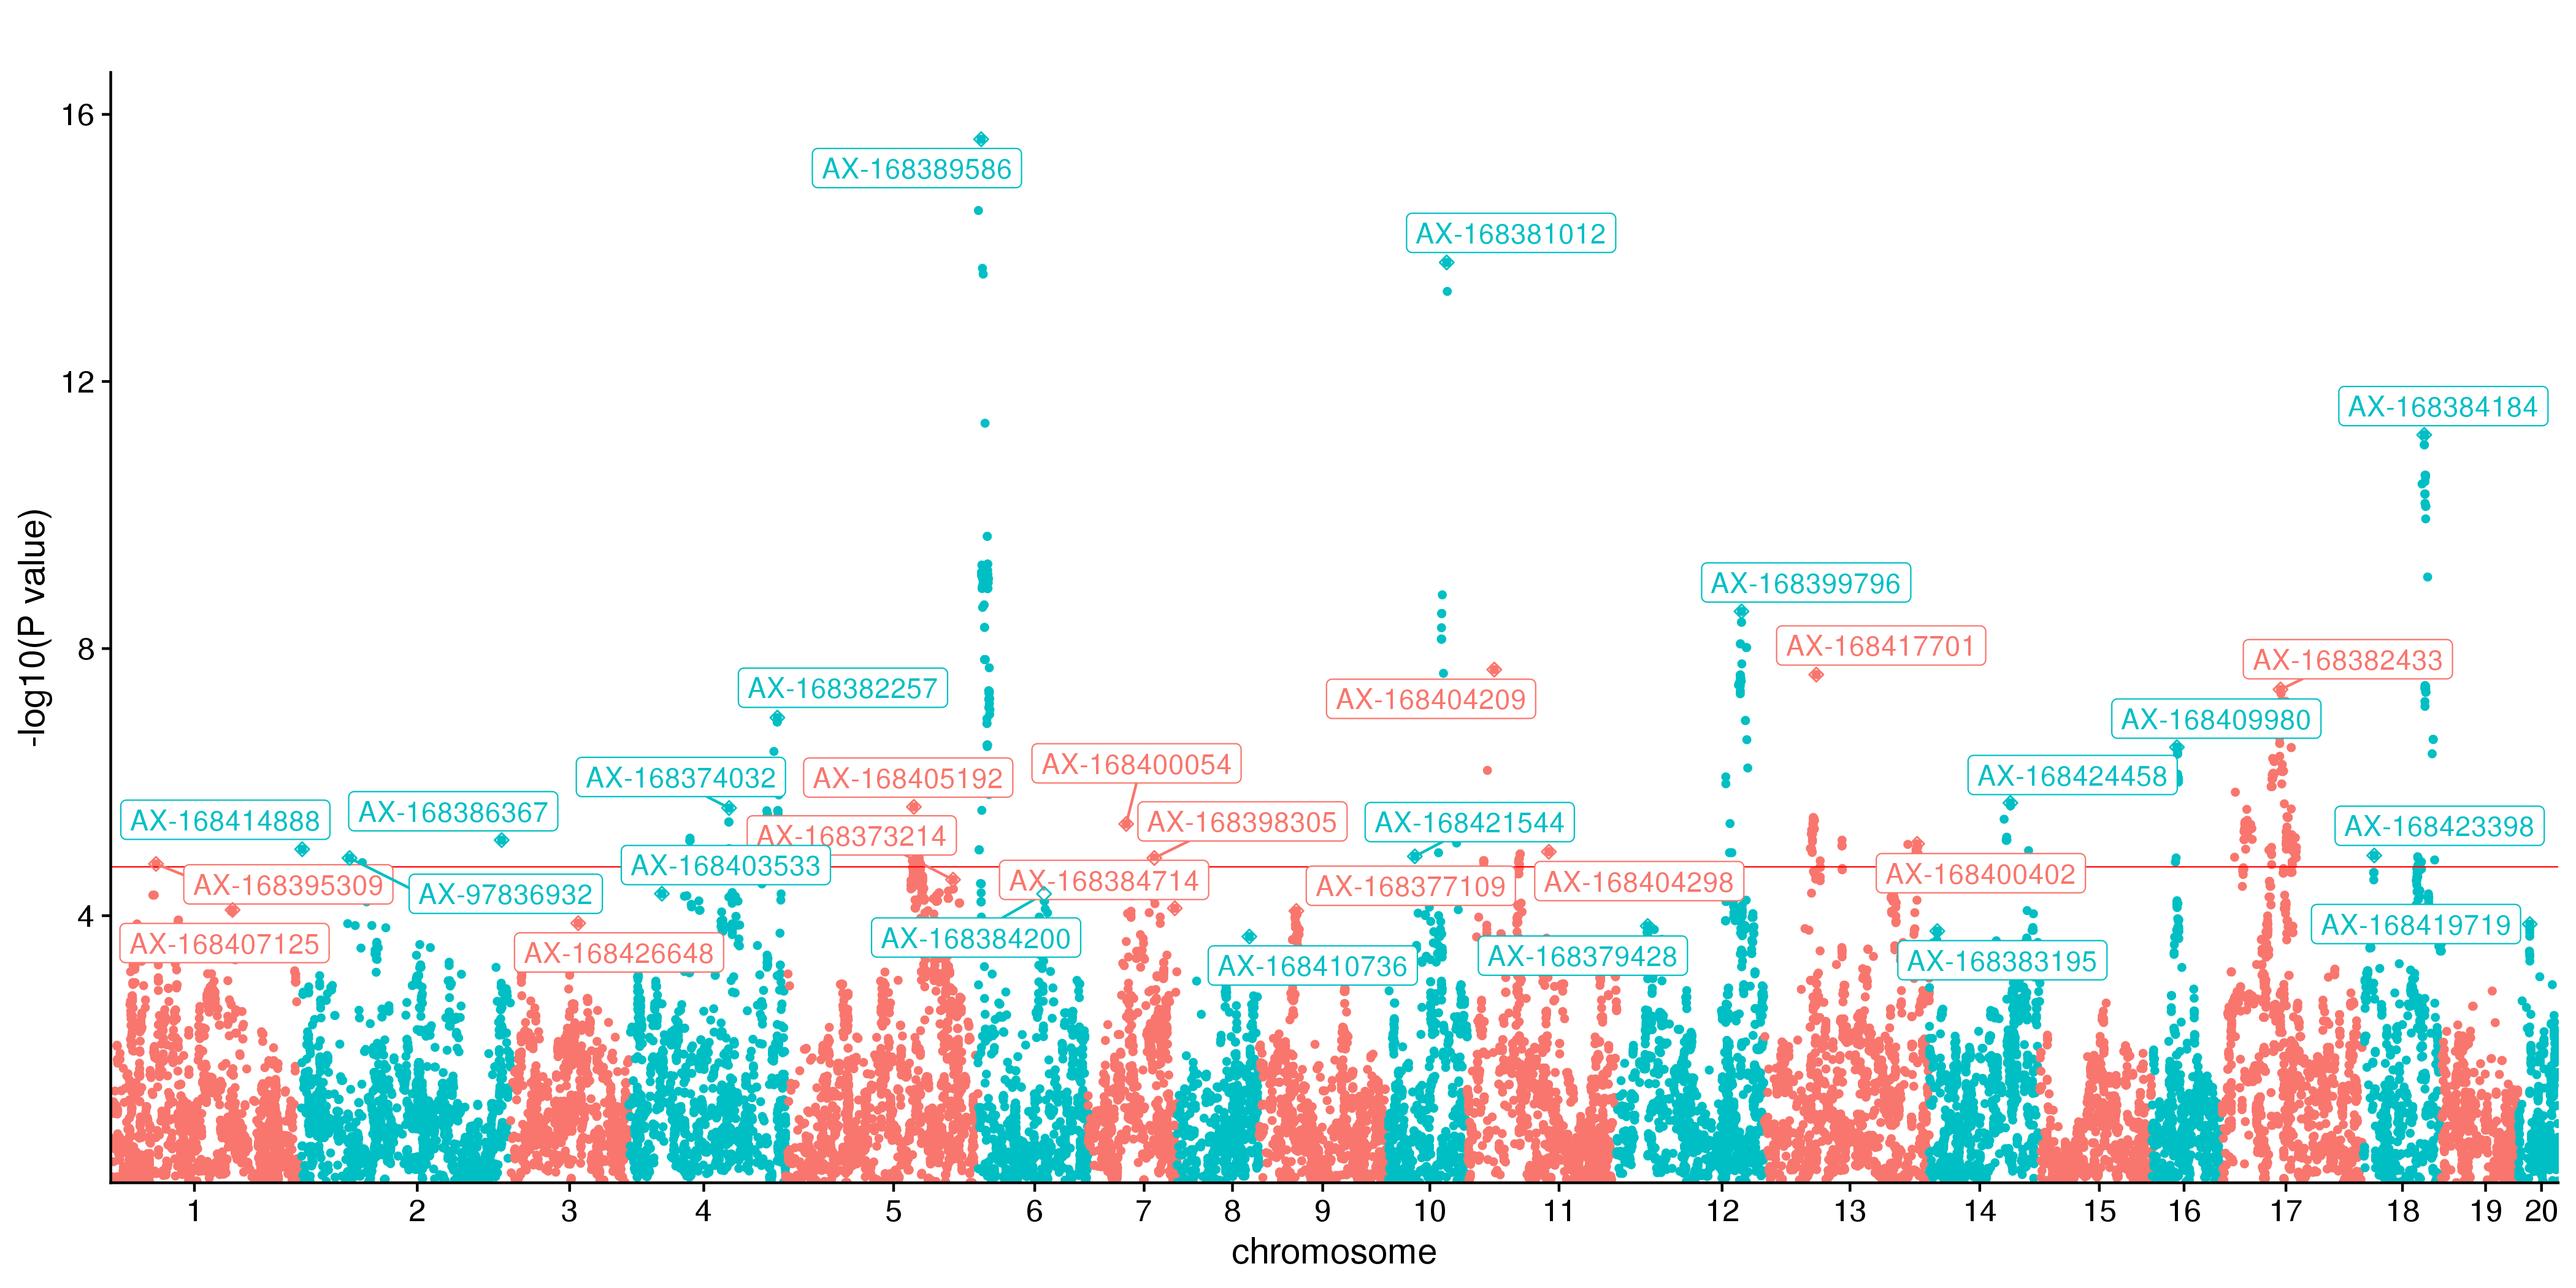
\includegraphics[width=\linewidth]{chapter_atchley/media/selected_snps.png}
    \caption[Manhattan plot multivariate growth]{Manhattan plot for the p-values in the QTL mapping. Significant SNPs that were selected for analysis are labeled by their ID in the SNP array. The red vertical line marks the corrected 5\% genome-wide significance threshold. Alternating colors separate the chromosomes.}
    \label{manhattan}
\end{figure}

\begin{table}[ht]
\centering
\caption[List of mapped loci]{Pleiotropic QTL, their locations in the genome, significance and classification using putative Early-Late modular hypothesis. P-values marked with an * are also significant at the genome-wide level.}
\label{qtltable}
\begin{tabular}{rlrrrlr}
  \hline
 & SNP ID & Chromosome & Position (bp) & Position (cM) & Classification & $-log_{10}(\text{p-value})$ \\ 
  \hline
1 & AX-168395309 &   1 & 49057268 & 25.84 & Modular & 4.77 \\ 
  2 & AX-168407125 &   1 & 125983982 & 54.05 & Intra-module & 4.09 \\ 
\midrule
  3 & AX-168414888 &   2 & 3732610 & 2.18 & Intra-module & 4.99 \\ 
  4 & AX-97836932 &   2 & 44187081 & 26.82 & Antagonistic & 4.86 \\ 
  5 & AX-168386367 &   2 & 174150478 & 97.91 & Intra-module & 5.13* \\ 
\midrule
  6 & AX-168426648 &   3 & 92533605 & 40.16 & Modular & 3.89 \\ 
\midrule
  7 & AX-168403533 &   4 & 35547379 & 17.62 & Antagonistic & 4.33 \\ 
  8 & AX-168374032 &   4 & 101163884 & 46.88 & Intra-module & 5.61* \\ 
  9 & AX-168382257 &   4 & 148270976 & 78.87 & Intra-module & 6.97* \\ 
\midrule
  10 & AX-168405192 &   5 & 101942137 & 48.76 & Local & 5.63* \\ 
  11 & AX-168373214 &   5 & 132074919 & 71.04 & Integrated & 4.54 \\ 
\midrule
  12 & AX-168389586 &   6 & 7605170 & 3.33 & Integrated & 15.63* \\ 
  13 & AX-168384200 &   6 & 91114085 & 40.39 & Antagonistic & 4.33 \\ 
\midrule
  14 & AX-168400054 &   7 & 63635159 & 33.46 & Antagonistic & 5.37* \\ 
  15 & AX-168398305 &   7 & 108326895 & 54.50 & Integrated & 4.86 \\ 
  16 & AX-168384714 &   7 & 140803834 & 77.20 & Intra-module & 4.11 \\ 
\midrule
  17 & AX-168410736 &   8 & 114057523 & 58.02 & Modular & 3.69 \\ 
\midrule
  18 & AX-168377109 &   9 & 38023383 & 20.83 & Intra-module & 4.07 \\ 
\midrule
  19 & AX-168421544 &  10 & 45619439 & 23.98 & Intra-module & 4.89 \\ 
  20 & AX-168381012 &  10 & 97173547 & 50.38 & Modular & 13.78* \\ 
\midrule
  21 & AX-168404209 &  11 & 24848821 & 15.27 & Intra-module & 7.69* \\ 
  22 & AX-168404298 &  11 & 68016486 & 41.60 & Antagonistic & 4.96 \\ 
\midrule
  23 & AX-168379428 &  12 & 27600863 & 9.80 & Antagonistic & 3.85 \\ 
  24 & AX-168399796 &  12 & 101775963 & 50.85 & Modular & 8.56* \\ 
\midrule
  25 & AX-168417701 &  13 & 40086090 & 19.44 & Modular & 7.61* \\ 
  26 & AX-168400402 &  13 & 111302641 & 62.25 & Integrated & 5.08* \\ 
\midrule
  27 & AX-168383195 &  14 & 16548147 & 7.04 & Antagonistic & 3.77 \\ 
  28 & AX-168424458 &  14 & 93468184 & 45.79 & Integrated & 5.69* \\ 
\midrule
  29 & AX-168409980 &  16 & 37004375 & 26.16 & Intra-module & 6.52* \\ 
\midrule
  30 & AX-168382433 &  17 & 41058707 & 19.56 & Integrated & 7.39* \\ 
\midrule
  31 & AX-168423398 &  18 & 15430276 & 8.63 & Intra-module & 4.90 \\ 
  32 & AX-168384184 &  18 & 71316734 & 45.02 & Integrated & 11.20* \\ 
\midrule
  33 & AX-168419719 &  20 & 52242051 & 29.97 & Antagonistic & 3.87 \\ 
   \hline
\end{tabular}
\end{table}

\begin{figure}
    \centering
    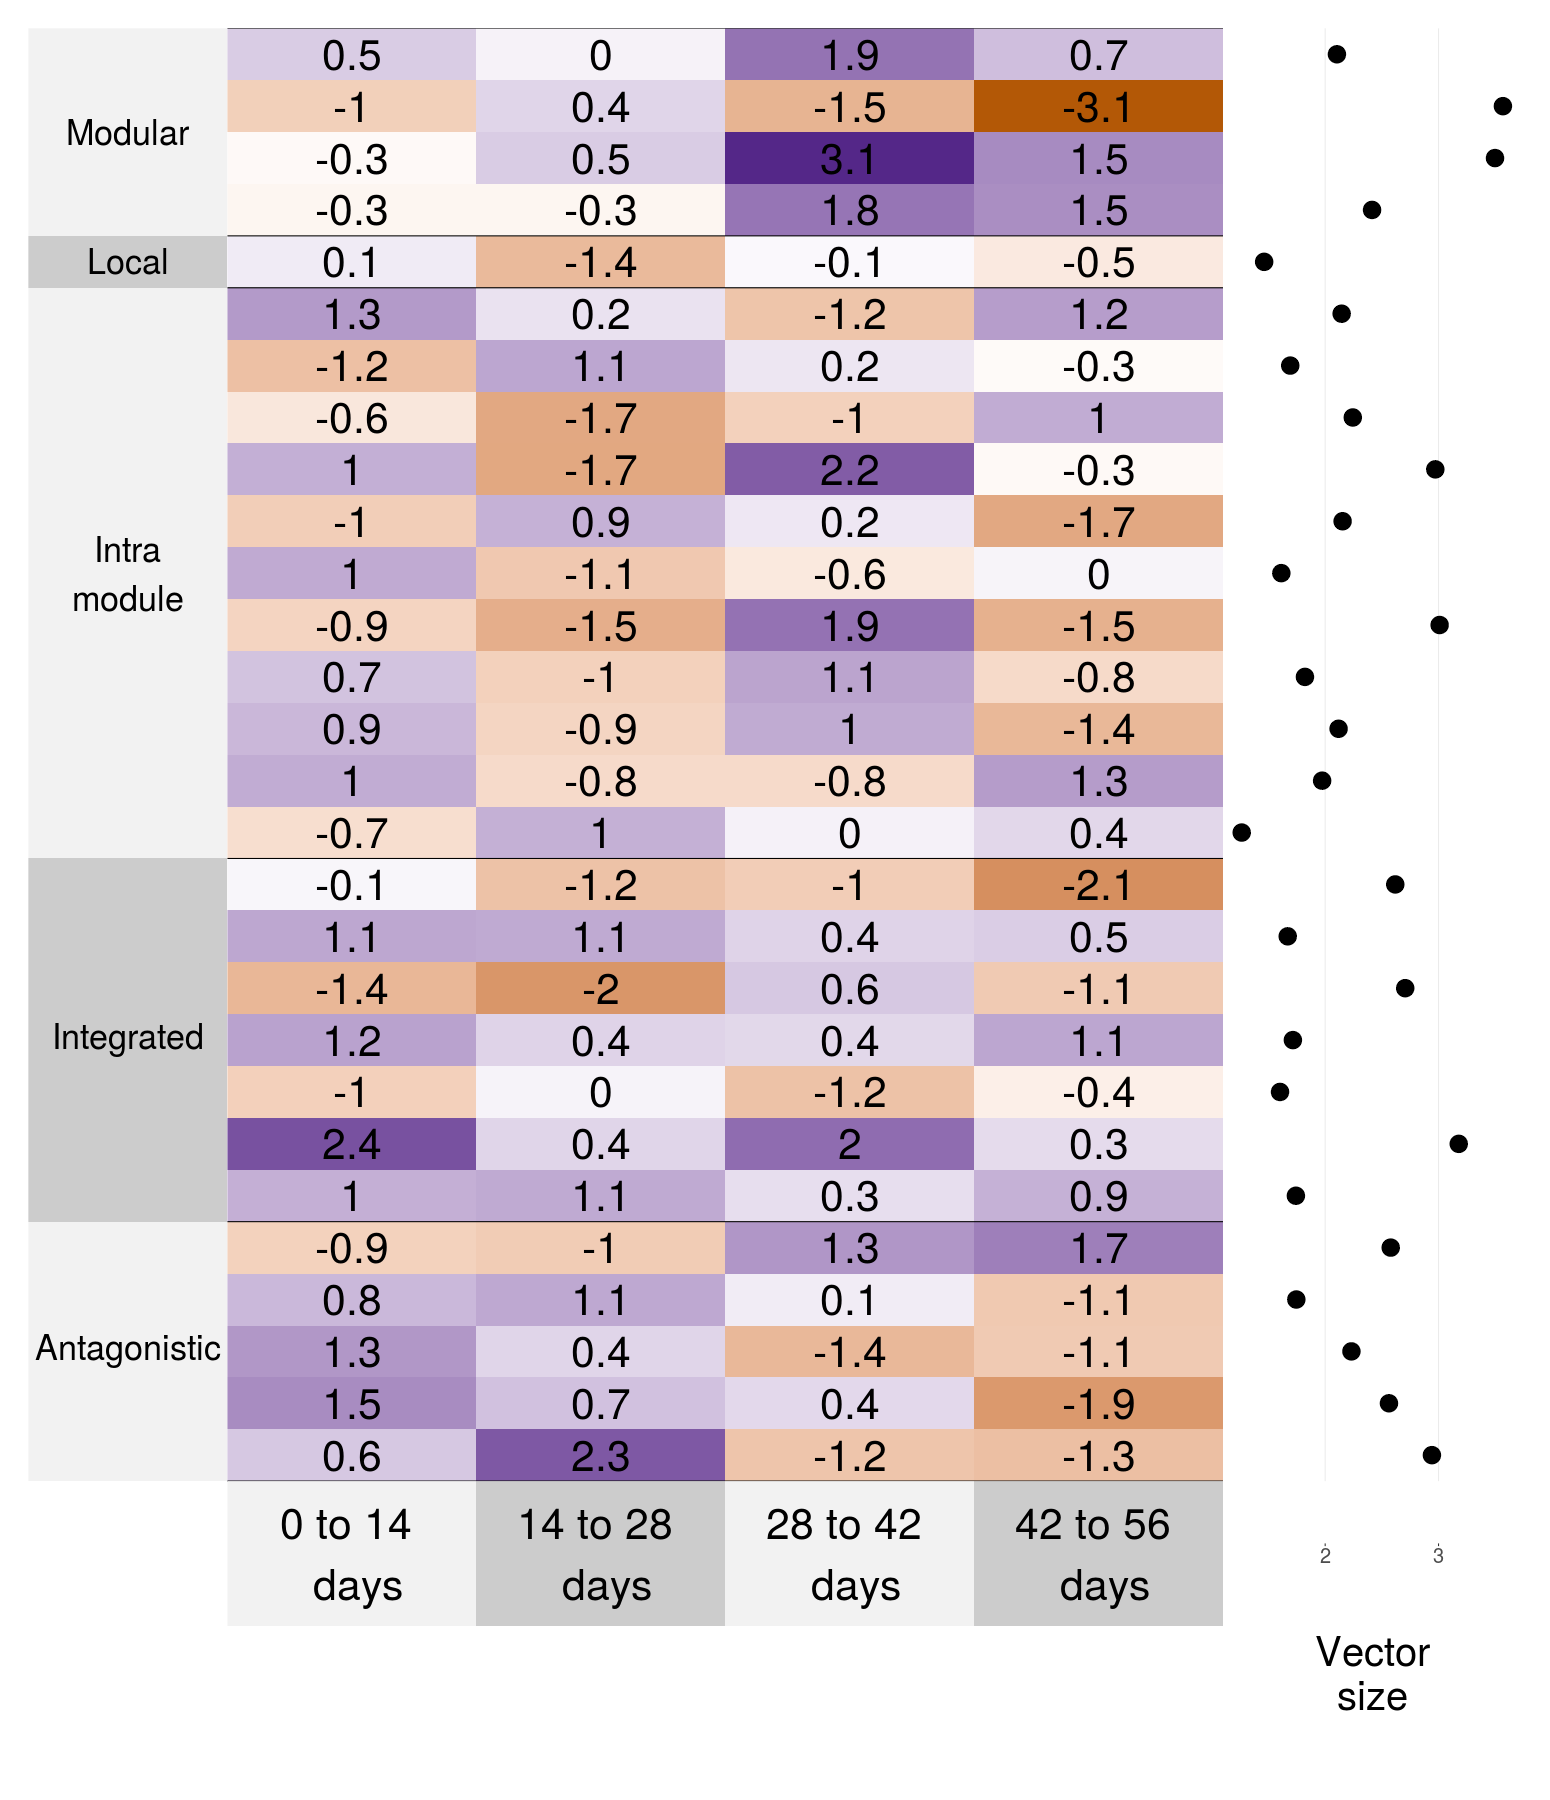
\includegraphics[width=\linewidth]{chapter_atchley/media/additive_effects_points.png}
    \caption[QTL effect classification]{Additive effects mapped using multivariate GWAS. 
    Each significant marker is associated with a pleiotropic effect vector, and these vectors 
    are classified into the genetic effect classes using alignment with a putative Early-Late 
    modular pattern. Color indicates the sign of the effect, and points show the overall magnitude 
    of the pleiotropic effect. Effects are scaled by trait standard deviation and multiplied by 10.}
    \label{additive_effects_vectors}
\end{figure}

\begin{figure}
    \centering
    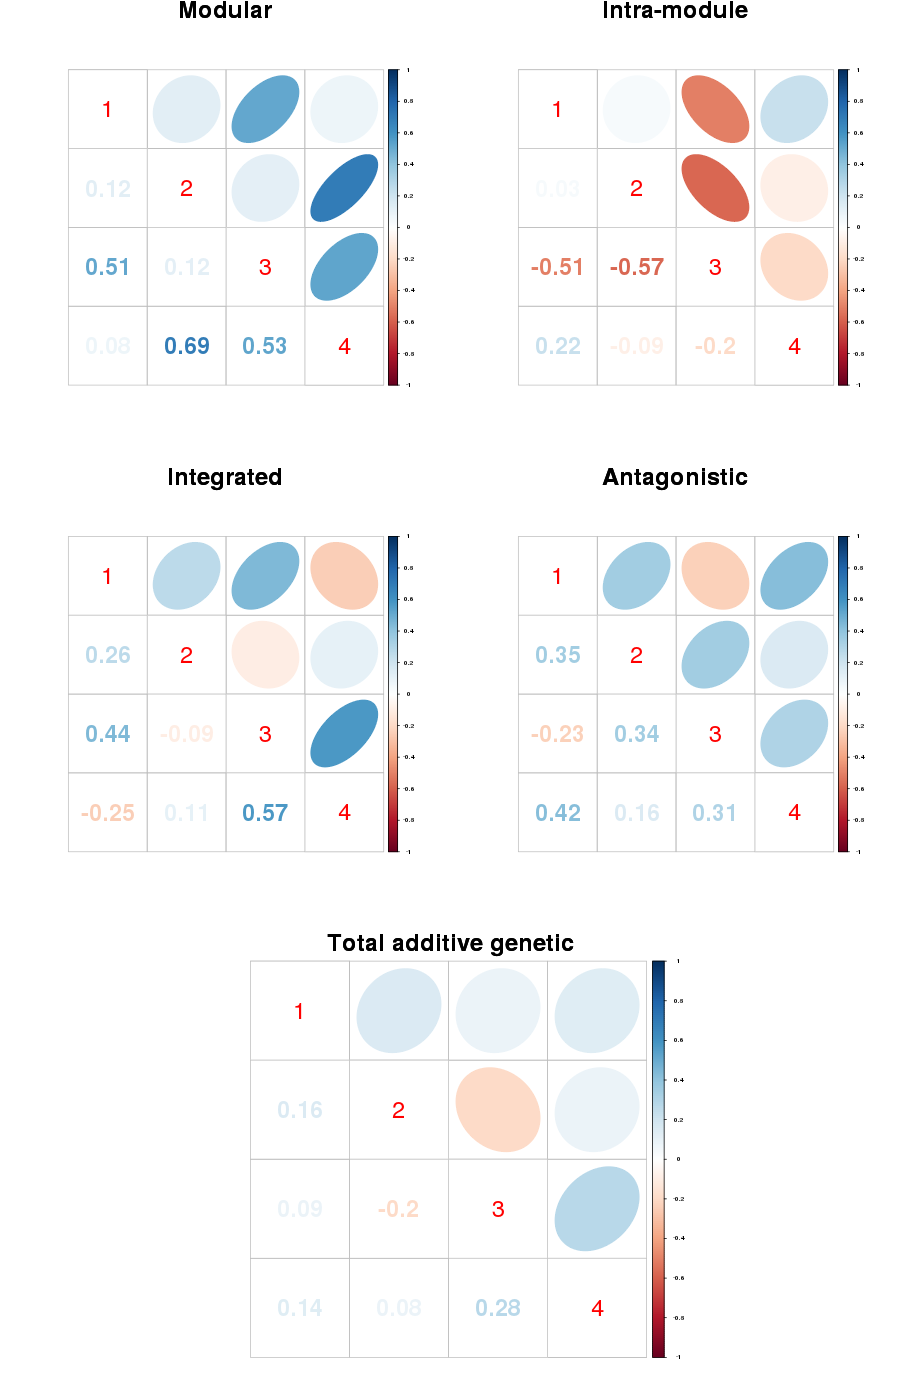
\includegraphics[width=\linewidth]{chapter_atchley/media/additive_matrices_by_class.png}
    \caption[Covariance matrices by effect class]{}
    \label{additive_effects_matrices}
\end{figure}


\section{Discussion}

In this manuscript we used simulations and an advanced intercross to study the
additive contribution of pleiotropy to the establishment of a new genetic
covariance pattern. We use simulations and an advanced intercross line and QTL
mapping to explore the additive genetic architecture underlying the observed
covariance pattern. Even when focusing only on the additive portion of the
genetic effects, both simulations and QTL mapping show a complex pattern of
modular and antagonistic effects that make up the observed covariation. This
underscores the difficulty in uncovering patterns of pleiotropy from genetic
covariation alone~\parencite{Mitteroecker2007-xq, Mitteroecker2009-jb}.

In the simulations, both stabilizing and directional selection are efficient
at creating variational modularity. All simulated populations share a similar
two-module correlation pattern, but the genetic basis of this modular
pattern can change depending on the evolutionary history of the population.
In general, a combination of modular, integrative and antagonistic genetic
effects interact to produce the final modular variational pattern, but
directional selection can increase the proportion of effects aligned with it,
altering the GP-map. In particular, the populations under directional
selection show an enrichment for pleiotropic effects that are in the same
direction as the directional selection. Divergent directional selection
produces a population with more antagonistic effects, while corridor selection
produces and excess of modular effects.

 In the advanced intercross line, the F$_{\text{5}}$F$_{\text{6}}$ generation shows a pattern of covariation in growth that is markedly different from the original mice that underwent divergent directional selection~\parencite{Atchley1997-vn}, with the erosion of a positive correlation between Early and Late growth. This reduction in covariation under directional selection is compatible with what we see in the simulated populations. 

Using an experimental cross, we see that the modularity pattern created by a divergent selection regime can be more complex, suggesting additional restrictions like development and correlated mutations also play a role in shaping restrictions. This covariation pattern is also created by a combination of several types of genetic effects, showing that simple "modular" or "pleiotropic" patterns are a simplification and that we need to consider complex GP-maps to understand the evolution of genetic restrictions.

What we predict, what we miss:
- Within module correlations are largely positive in most genetic effect classes. 
- General pattern is predicted by the SNPs, but correlations are lower and we miss a negative correlation.
- Intra-module contribute to the negative correlations
- Missing dominance effects could have a large contribution to the observed negative correlation.
- Across line correlation is zero, not negative, supporting the role of interactions.

- Plenty of variation in covariance pattern.
- Variation comes from multiple types of effects, not necessarily aligned with selection. 
- Covariance is created by complex genetic architecture, not simple "modularity" or "hidden pleiotropy".
- Other studies on the congruence between pleiotropy and covariation: 

- \parencite{Porto2016-qc} 

- \parencite{Leamy2002-nh}

- \parencite{Kenney-Hunt2008-bd}

- \parencite{Jones2014-wj}

- \parencite{Chebib2017-sv}

Pavlicev Phillip Dominance in the skull, Chevin on mutational variation.

\printbibliography

\end{refsection}